\documentclass[11pt, letterpaper]{article}
\usepackage{amsmath}
\usepackage{caption}
\usepackage{color}
\usepackage{float}
\usepackage{fullpage}
\usepackage{graphicx}
\usepackage{longtable}
\usepackage{multirow}
\usepackage[nottoc]{tocbibind}
\usepackage{subcaption}
\usepackage{url}
\setlength{\pdfpagewidth}{\paperwidth}
\setlength{\pdfpageheight}{\paperheight}
\setcounter{tocdepth}{2}

\renewcommand{\captionfont}{\small}

\newcommand{\degrees}{$^{\circ}$ \,}
% \newcommand{\question}[1]{\textbf{#1}}

\begin{document}
\title{\textbf{Title}\\
{\Large Ph.D. Thesis}}
\author{Ronald J. Nowling}

\maketitle

\newpage

\tableofcontents

\newpage

\chapter{\uppercase{Introduction}}

Arthropod vectors are increasingly becoming important in emerging human disease outbreaks.  In addition to the recent Zika outbreak vectored by the mosquito \emph{Aedes aegypti}, linked to serious medical outcomes, nearly half of the world's population is still at risk of contracting malaria.  In 2015, 214 million malaria infections, resulting in 438,000 deaths, were reported. Nearly 90\% of the reported infections and deaths have occurred in Sub-Saharan Africa.  Mosquitoes in the \emph{Anopheles} genus are the sole vectors of the malaria-causing \emph{Plasmodium} parasites \cite{Neafsey2015,Neafsey2010,Lawniczak2010}. As such, efforts to control populations of insect vectors such as \emph{Anopheles gambiae} are key to efforts to eradicate malaria and other insect-borne diseases \cite{Holt2002}.

\emph{Anopheles} species have been subject to evolutionary adapations due to host-parasite interactions and specializations needed to thrive when living among and feed on humans \cite{Neafsey2015}. Population control efforts are informed through studies of insect biology and characterizerations of these adaptations, which are enabled by sequencing and comparative analysis of insect genomes.   Such studies have been fruitful, with results including the identification of chemosensory receptors responsible for detection of human hosts and the molecular bases of variations in insecticide resistance between populations and species \cite{Lawniczak2010}.

Bioinformatic analysis of insect genomes is complicated by unique characteristics of insect biology.  For example, mammalian chemosensory receptors are G Protein Coupled Receptors (GPCRs), while insect chemosensory receptors are ion channels which are poorly-conserved on the sequence level \cite{Sato2008,Touhara2009,Wicher2008}.  Insect genomes tend to have low linkage disequilibrium (LD), or correlation  between variations located nearby on chromosomes, resulting in low statistical power when identifying interesting variations.

The larger bioinformatics community is adept at developing algorithms and accompanying software to meet such challenges.  Developing methods and software is expensive in terms of time and resources (human, financial), however. A majority of bioinformatics software is developed for a single or small number of analyses, abandoned once the analyses are done. Studies of defect rates in software have found that bugs tend to most frequently occur in files with the most recent activity \textcolor{red}{cite}.  Interpreted another way, new bugs can be introduced in the process of adding new features and fixing previously-known bugs can; over time, however, modules mature and the rate at which new bugs are found declines, leading to reliable components. Furthermore, bioinformatics applications often employ specalized methods not available in common libraries.  As such, bioinformatics software often consists of completely custom implementations of every component from file parsers to complex algorithms and statistical tests.  We can conclude that most bioinformatics applications consist of new, custom code with high defect rates, leading to significant development costs due to time spent debugging.

Furthermore, bioinformatics software is often used on large data sets and employs computationally-expensive algorithms.  Since reducing software run times from hours or days to minutes can significantly boost productivity, enabling a much shorter loop in idea-implementation-evaluation cycles, it is highly desireable to optimize and parallelize code.  Low-level languages like C are often used to achieve optimal usage of hardware. C is more error-prone than high-level langauges like Python, however, due to manual memory management and poor type safety.  Parallelization is also known to increase software complexity and defect rates, especially since race conditions are notoriously difficult to debug. Both requirements lead to increased time and effort spent debugging and validating software.

Machine learning libraries offer an attractive alternative.  Due to general applicability, machine learning techniques are widely applied through academia and industry.  A number of mature and widely-used machine learning libraries exist including the scikit-learn \cite{scikit-learn} library for Python and the MLLib library bundled with the Apache Spark distributed-computing engine.  As of the time this was written, scikit-learn and Apache Spark have been around for 8 and 7 years, over 550 and 1,000 contributors, and over 2,600 and 1,100 citations, respectively. Both libraries implement a number of popular machine learning techniques including Random Forests, K-Means clustering, Support Vector Machines (SVMs), and Naive Bayes classifiers. 

The machine learning community is also adept at scaling computationally-complex algorithms to large data sets; scikit-learn and MLLib offer best-in-class performance and scalability.  Scikit-learn is optimized via C and Fortran implementations of performance-critical sections and can efficiently scale through support for parallel processing.  Through Apache Spark and conscientious design, MLLib can scale from a single machine to a large cluster to support data sets too large to fit into memory and algorithms too slow to use productively when running on a single CPU core. Users of scikit-learn and MLLib reap the resulting performance and scalability benefits essentially for free; the libraries largely hide the details from the user.

By adopting machine learning techniques as building blocks for developing bioinformatics methods and applications, machine learning libraries could be adopted, benefitting method developers. Software defects tend to be over-represented in functions employing complex algorithms, parallelization, and low-level optimizations like manual memory management, exactly the functionality that would be replaced by the machine learning libraries, presumably decreasing defect rates and time and labor spent debugging. Additionally, scaling software to large data sets and achieving optimal hardware utilization could be accomplished with far less effort; the optimizations and parallelization techniques employed by machine learning libraries are hidden completely from the user or accomplished by through abstractions that are easier to use.

\section{Contributions}
Prerequisite is to demonstrate that machine learning techniques are applicable to problems in bioinformatics and just as, if not more, effective when replacing or augmenting specialized techniques.  In this dissertation, we consider several of the unique challenges facing bioinformatics of insect genomes and apply machine learning to two common problems in bioinformatics, finding members of a gene family in genomes and ranking genetic variants based on association with population structures.  We demonstrate that both problems are instances of classic machine learning problems, classification and feature selection, respectively.

First, we describe analyzes of the genomes and RNASeq expression of genes from two sand fly species, \emph{Lutzomyia longipalpis} and \emph{Phlebotomus papatasi}, which are vectors of leishmaniasis.  We utilized four analyses to compare the genomes: genome assembly completeness, conservation of gene order (synteny), distributions of ratios of non-silent to silent mutations ($d_N$/$d_S$) in single-copy orthologs, and differential expression of genes in \emph{L. longipalpis} females under sugar-fed, blood-fed and infected-blood fed condition with RNASeq.  Our analysis identified differential expression and synteny blocks of peritrophins, chitinases, and Niemann-Pick type C-2 (NPC2) genes associated with vector-parasite interactions. Peritrophin matrices enable the \emph{Leishmania} parasites in the bloodmeal to survive the digestive process.  Chitinases breakdown the peritrophix matrix, allowing the parasites to escape and remain within in the vector.  NPC2 genes are involves in sterol and sex hormone homeostatis and have been linked to a diverse range of functions including the insect's immune system. These analyses provide examples of the types of questions that biologists seek to answer and the challenges associated with insect genome bioinformatics.  

Secondly, we describe a novel ensemble approach for identifying G Protein-Coupled Receptors (GPCRs) in insect vector genomes.  As part of a genome analysis, genes are annotated and their functionality predicted based on known orthologs. GPCRs possess low levels of sequence conservation, spawning research into methods that can provide more accurate identification and classification than BLAST alone.  Existing GPCR classifiers such as GPCRHMM and PredCouple present several limitations: the classifiers have been trained using GPCRs from a diverse set of model organisms including human (\emph{Homo homo sapiens}) and the fruit fly \emph{Drosophila melanogaster}, resulting in sub-optimal performance when applied to evolutionarily-distance, non-model insect vectors and their scoring systems can be difficult to interpret.  We describe a novel pipeline, called Ensemble*, that combines GPCRHMM, Pfam GPCR Hidden Markov Models (HMMs), and empirical conditional probability functions to improve sensitivity, accuracy, and interpretability over GPCRHMM and Pfam HMMs alone. We evaluated the sensitivity and accuracy of GPCRHMM, PredCouple, the Pfam GPCRH HMMs, and Ensemble*, demonstrating improved sensitivities of up to 10\% on \emph{Aedes aegypti}, \emph{Anopheles gambiae}, \emph{Apis mellifera}, and \emph{Pediculus humanus} with no loss of sensitivity for \emph{Drosophila melanogaster} and \emph{Homo homo sapiens}. Using Ensemble*, we re-analyzed the GPCR repoirteres of the vectors \emph{Aedes aegypti}, \emph{Anopheles gambiae}, resulting in the identification of 30 additional putative GPCRs, of which 19 were validated and confirmed via sequence similarity to known GPCRs with BLAST.

Lastly, we describe a workflow for ranking SNPs from incipient \emph{Anopheles} species using Random Forests.  Separated populations of insect vectors are often compared to identify the genetic basis for differences in insecticide resistance, host preferences, and ecological adaptations.  We demonstrated that Random Forests can be used successfully to rank SNPs in terms of their association with a given population structure.  We identified several causes of bias using numerical experiments and describe appropriate solutions that can be used with standard, \emph{unmodified} implementations of decision trees available in popular machine learning libraries. We provided a software package called Asaph that implements the workflow using Python, numpy, scipy, and scikit-learn.  Asaph was applied to SNPs from \emph{Anopheles gambiae}, \emph{Anopheles coluzzii}, and two forms of \emph{Anopeheles funestus}, Folonzo and Kiribina, resulting in the identification of SNPs in genes previously reportedly to be associated with differences in insecticide resistance between the populations.

Our comparative genomic analysis of \emph{P. papatasi} and \emph{L. longipalpis} provides examples of analyses used by bioinformaticians studying insect vectors.  Ensemble* demonstrates that machine learning techniques can be used to augment existing bioinformatics tools to achieve higher sensitivity and accuracy when applied to new data sets, avoiding the need to develop new methods from scratch. And, lastly, by applying Random Forests to identifying biologically-interesting SNPs in a population genetics framework, we demonstrated that machine learning techniques can replace traditional domain-specific techniques, opening the door to using existing machine learning libraries to simplify bioinformatics application development.

\section{Synopsis}
The rest of this dissertation is organized as follows:

\begin{itemize}
\item Chapter 2: Comparative analysis of the genomes of and RNASeq expression of genes from two sand fly species, \emph{L. longipalpis} and \emph{P. papatasi}.
\item Chapter 3: Evaluation of Hidden Markov Model (HMM)-based tools for identifying G Protein-Coupled Receptors (GPCRs) in insect vector genomes and demonstratation of how a simple approach for creating an ensemble of existing classifiers can improve accuracy by at least 5-11\%.
\item Chapter 4: Application of Random Forests to ranking SNPs from incipient species of \emph{Anopheles} mosquitoes.  We identify multiple sources of bias that can arise and provide solutions that utilize ``out-of-the-box'' implementations of decision trees.  We provide a software implementation of our workflow using the popular machine learning library sci-kit learn, which we apply to the study of SNPs from several \emph{Anopheles} species.
\end{itemize}

We conclude by identifying topics for further investigation.

\pagebreak
\section{GPCR Classifier}
\pagebreak
\chapter{Characterization and Automated Detection of Insect Chemosensory Receptors}

\section{Introduction}

\section{Methods}

\subsection{Data Sets}

Protein sequences for known chemosensory receptors from 12 \emph{Drosophila} and 3 mosquito species (\textcolor{red}{TODO TABLE}) were downloaded from their respective databases.

The chemosensory receptor protein sequences from the 12 species of \emph{Drosophila} and 3 species of mosquitoes were separated into separate sets of olfactory and gustatory receptors.

\textcolor{red}{TODO how were these sequences identified?}

\subsection{Characterization of Amino Acid Conservation}
Clustal-$\Omega$ (\textcolor{red}{TODO CITE, version}) was used to perform separate multiple sequence alignments (MSAs) of the olfactory and gustatory receptors from the 12 species of \emph{Drosophila} and 3 species of mosquitoes.  \textcolor{red}{TODO REMOVE outliers}.  The observed frequencies of each amino acid was computed for each position in the MSAs.  The maximum frequency and its associated amino acid was found for each position.  The maximum frequencies were plotted to identify highly-conserved residues.

\subsection{Identification Approach 1: Digrams, Weighting, and Clustering}

\subsection{Identification Approach 2: Profile Hidden Markov Models (HMMs)}

Clustal-$\Omega$ (\textcolor{red}{TODO CITE}) was used to perform separate multiple sequence alignments (MSAs) of the olfactory and gustatory receptors from the 12 species of \emph{Drosophila} and 3 species of mosquitoes.  The program \texttt{hmmbuild} from the HMMER (\textcolor{red}{TODO CITE, version}) package was used to build separate HMMs for the olfactory (OR HMM) and gustatory (GR HMM) receptors.  Two additional chemosensory HMMs (7tm\_6, 7tm\_7) were retrieved from the Pfam database \textcolor{red}{TODO CITE, version}) for a total of four HMMs.

The four HMMs were used to search the proteomes of the 12 \emph{Drosophila} and 3 mosquito species for chemosensory receptors using \texttt{hmmscan} from the HMMER (\textcolor{red}{TODO CITE, version}) package.  Each HMM was evaluated based on the number of olfactory and gustatory receptors correctly identified and other sequences incorrectly identified as potential chemosensory receptors.

Using \texttt{hmmscan} from the HMMER (\textcolor{red}{TODO CITE, version}) package, the four HMMs were used to search the proteome of \emph{D. suzukii} to find potential chemosensory receptors.  The resulting hits were validated by searching the NCBI nr database with \texttt{blastp} (\textcolor{red}{TODO CITE, version}).

\begin{figure}[H]
  \centering
  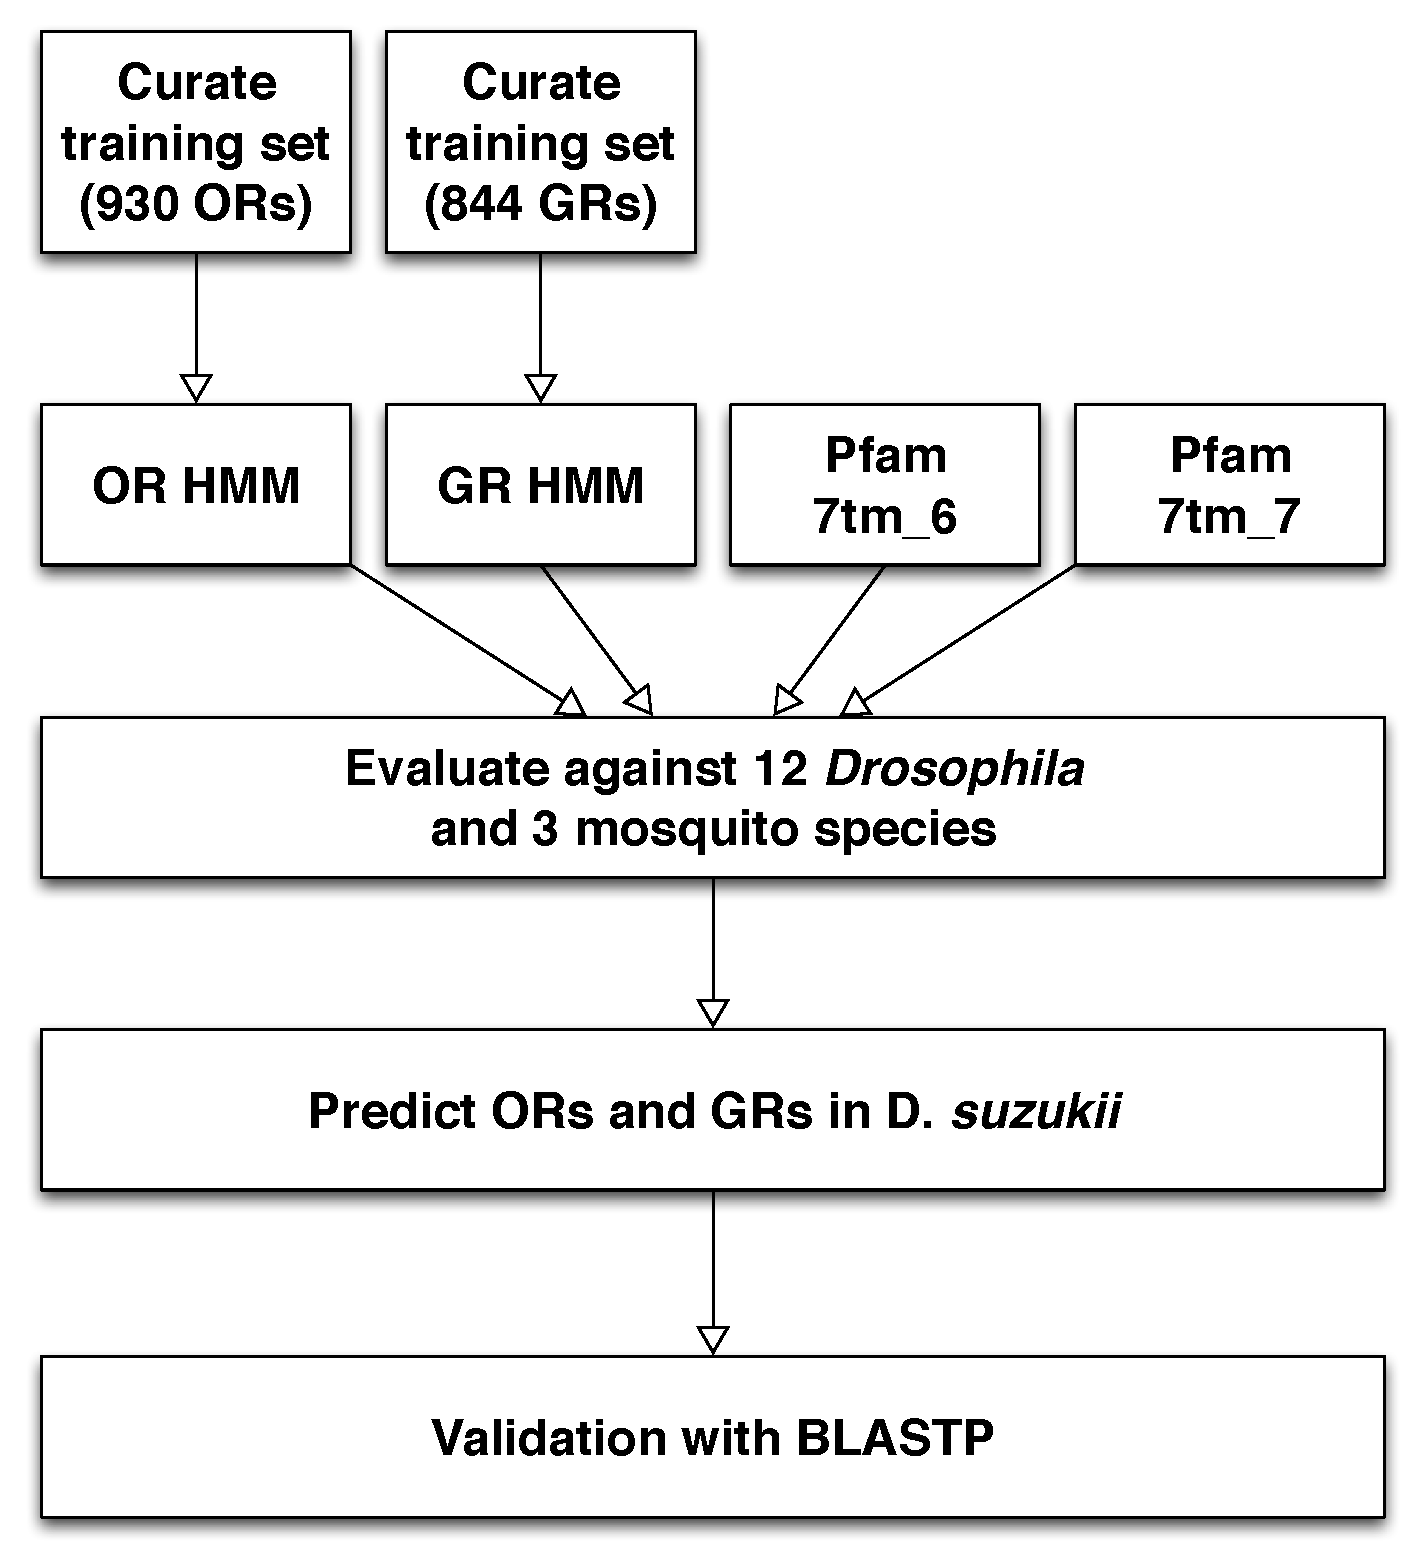
\includegraphics[width=0.7\textwidth]{figures/chemosensory/hmm_workflow}
  \caption{Workflow for HMM training, validation, and classification}
  \label{fig:chemosensory:hmm-workflow}
\end{figure}

\section{Results}

\subsection{Characterization of Insect Chemosensory Receptors}

\begin{figure}[H]
  \centering
  \begin{subfigure}[b]{0.45\textwidth}
    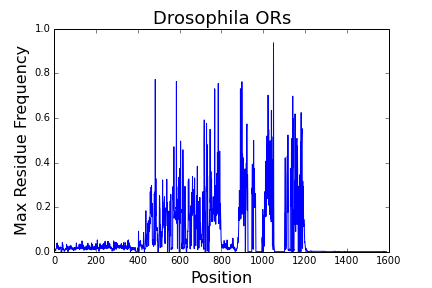
\includegraphics[width=\textwidth]{figures/chemosensory/drosophila_or_max_freq.png}
    \caption{Olfactory Receptors (930)}
    \label{fig:chemosensory:or-max-freq}
  \end{subfigure}
  ~
  \begin{subfigure}[b]{0.45\textwidth}
    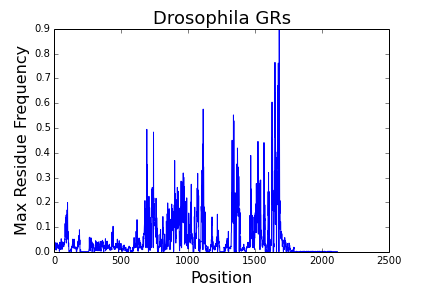
\includegraphics[width=\textwidth]{figures/chemosensory/drosophila_gr_max_freq.png}
    \caption{Gustatory Receptors (844)}
    \label{fig:chemosensory:gr-max-freq}
  \end{subfigure}
\label{fig:chemosensory:max-freq}
\caption{}
\end{figure}

\subsection{Comparing Approaches for Automated Identification}

\begin{table}[H]
  \centering
  \begin{tabular}{c c c c} \hline
  \emph{HMM} & \emph{Olfactory Receptors} & \emph{Gustatory Receptors} & \emph{Others} \\ \hline
  7tm\_6 & 881 & 15 & 223 \\ \hline
  OR & 928 & 68 & 297 \\ \hline
  7tm\_7 & 213 & 829 & 580 \\ \hline
  GR & 131 & 828 & 271 \\ \hline
  \end{tabular}
  \caption{Predicted Proteins from 12 \textit{Drosophila} and 3 mosquito species}
  \label{tab:chemosensory:hmm-validation}
\end{table}

\subsection{Identification \& Validation of \emph{D. suzukii} Chemosensory Receptors}

\begin{table}[H]
  \centering
  \begin{tabular}{c c c} \hline
  & \emph{Olfactory Receptors} & \emph{Gustatory Receptors} \\ \hline
  Predicted & 64 & 52 \\ \hline
  Validated & 56 & 45 \\ \hline 
  \end{tabular}
  \caption{Predicted and Validated Proteins \emph{D. suzukii}}
  \label{tab:chemosensory:suzukii-predictions}
\end{table}

\subsection{Discussion and Conclusion}

\pagebreak
\section{Synteny}

\subsection{Introduction}

\subsection{Methods}

\subsubsection{Data sets}


The \emph{Ae. aegypti}, \emph{An. gambiae}, \emph{L. longipalpis}, and \emph{P. papatasi} \textcolor{red}{TODO VERSIONS} peptide translations were downloaded from Vectorbase \textcolor{red}{TODO CITE}, while the \emph{D. melanogaster} and \emph{D. simulans} peptide translations were downloaded from Flybase \textcolor{red}{TODO CITE}.

\textcolor{red}{table of versions}


\subsubsection{Calculation of Scaffold Gene CDF}
The gene counts of each genome's scaffolds were normalized by dividing the gene counts by the number of genes in that organism's genome. For each genome, the scaffolds were sorted by their gene counts largest to smallest.  A cumulative sum was computed over the normalized gene counts.   The normalized cumulative size of each scaffold was plotted. For genomes which had few scaffolds than the largest genome, the plots were extended to the largest number of scaffolds among all of the organisms with points of value 1.


\subsubsection{Generation of Dot Plots for Macrosynteny}
The identifiers, scaffolds, locations, and sense in the FASTA headers were extacted for each peptide sequence (Figure~\ref{fig:synteny-workflow}).  The protein IDs were cross-referenced with OrthoDB to group the proteins into ortholog groups.  Sequences without ortholog information or no orthologs in the other genomes and ortholog groups with many-to-many and one-to-many relationships were discarded.  The proteins were sorted along each scaffold by their starting coordinates, while scaffolds were ordered arbitrarily.  Scatter plots were generated by drawing dots at the positions of orthologous proteins.

\begin{figure}[H]
  \centering
  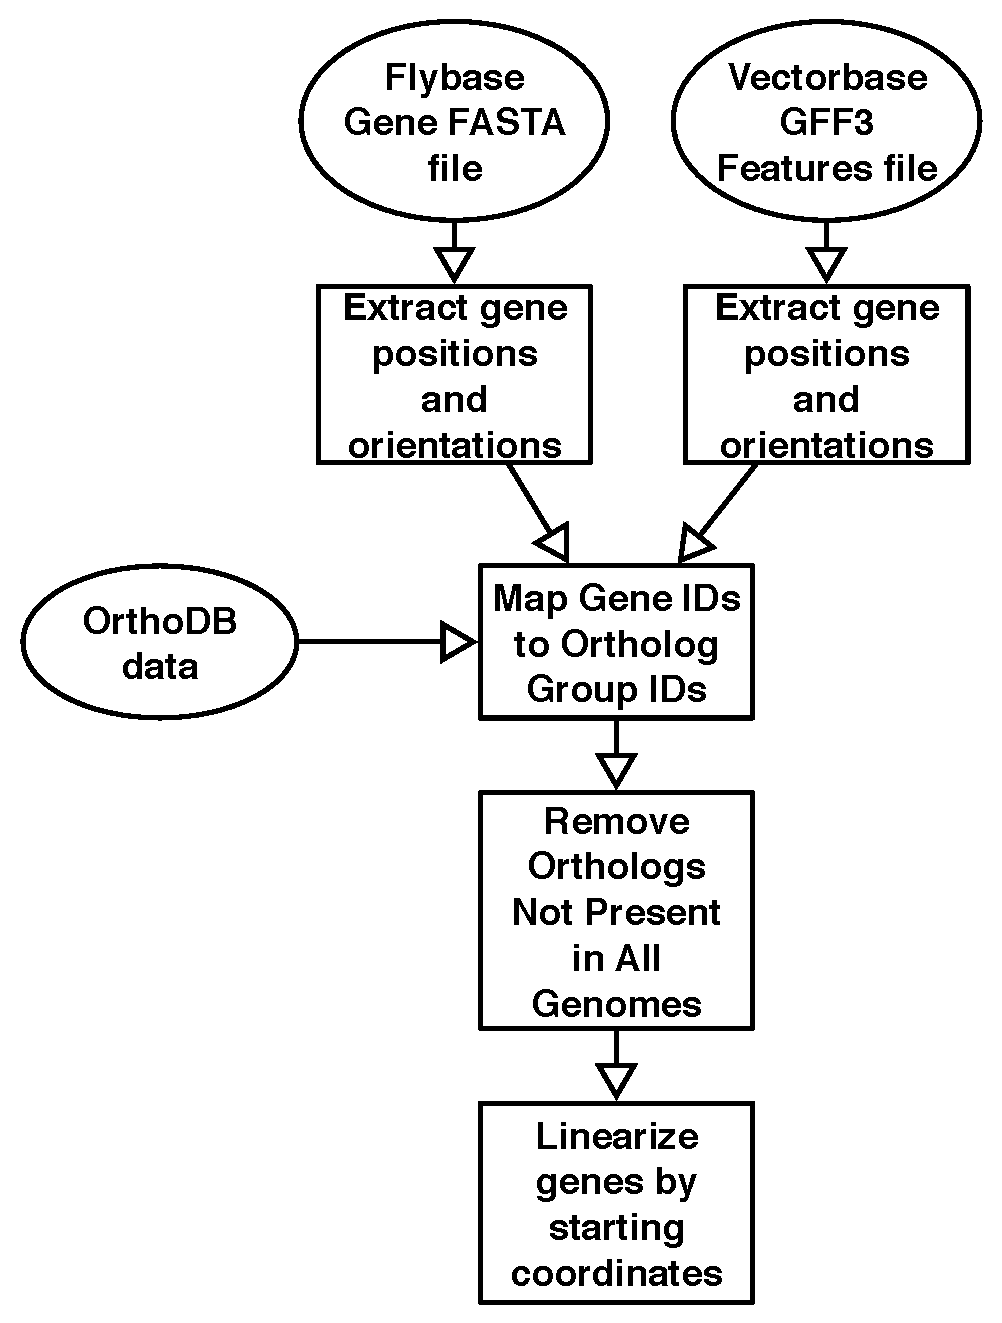
\includegraphics[width=0.5\textwidth]{figures/synteny/orthodb_dotplot_workflow}
  \caption{Workflow for Synteny}
  \label{fig:synteny-workflow}
\end{figure}

\subsubsection{Microsynteny}
For each genome, the identifiers, protein sequences, orientations, scaffolds, and locations extracted from FASTA files for each genome and reformatted as input for the program \texttt{Synchro} \textcolor{red}{TODO CITE}.  \texttt{Synchro} ($\Delta=5$) was run on the pairs \emph{D. melanogaster} and \emph{D. simulans}, \emph{An. gambiae} and \emph{L. longipalpis}, \emph{An. gambiae} and \emph{Ae. aegypti}, and \emph{L. longipalpis} and \emph{P. papatasi}.  Synteny blocks were extracted from the \texttt{OrthBlocks synt} files.  Three-way synteny blocks for \emph{An. gambiae}, \emph{L. longipalpis}, and \emph{P. papatasi} were constructed by finding all pairs of synteny blocks for \emph{An. gambiae} and \emph{L. longipalpis} and \emph{L. longipalpis} and \emph{P. papatasi} that overlapped by at least one gene.  

\textcolor{red}{TODO annotation of synteny blocks, distribution plots}


\subsection{Results}

\subsubsection{Genome Assembly Analysis}

\textcolor{red}{TODO DESCRIPTION}

\begin{figure}[H]
  \centering
  \begin{subfigure}[b]{0.45\textwidth}
    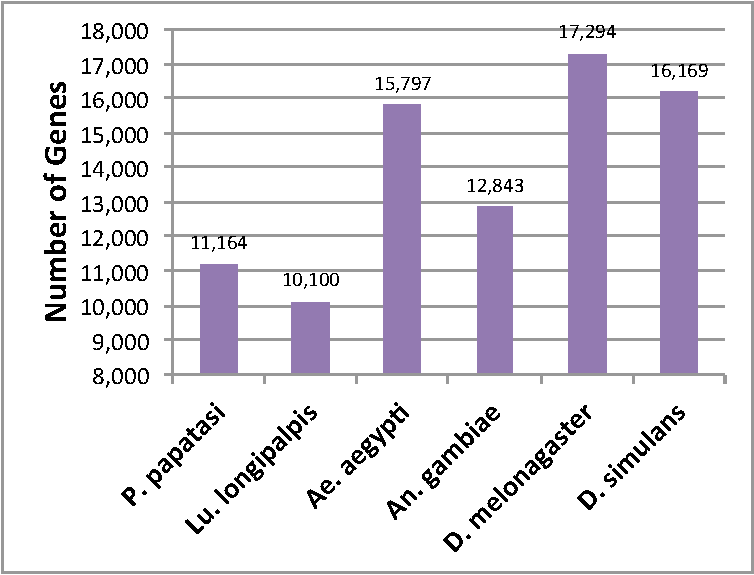
\includegraphics[width=\textwidth]{figures/synteny/genome_size_genes.pdf}
    \caption{Genome Sizes (Genes)}
  \end{subfigure}
  ~
  \begin{subfigure}[b]{0.45\textwidth}
    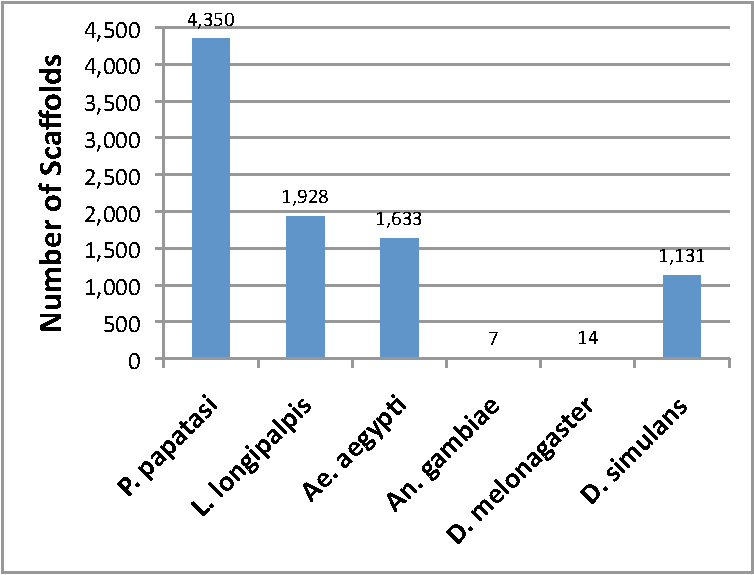
\includegraphics[width=\textwidth]{figures/synteny/scaffold_counts.pdf}
    \caption{Number of Scaffolds}
  \end{subfigure}
  ~
  \begin{subfigure}[b]{0.45\textwidth}
    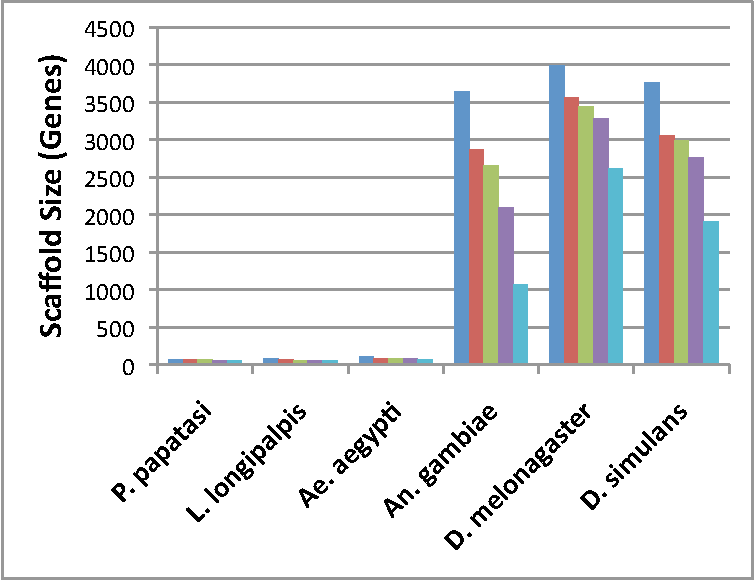
\includegraphics[width=\textwidth]{figures/synteny/top5_scaffold_sizes.pdf}
    \caption{Top 5 Scaffold Sizes (Genes)}
  \end{subfigure}
  ~
  \begin{subfigure}[b]{0.45\textwidth}
    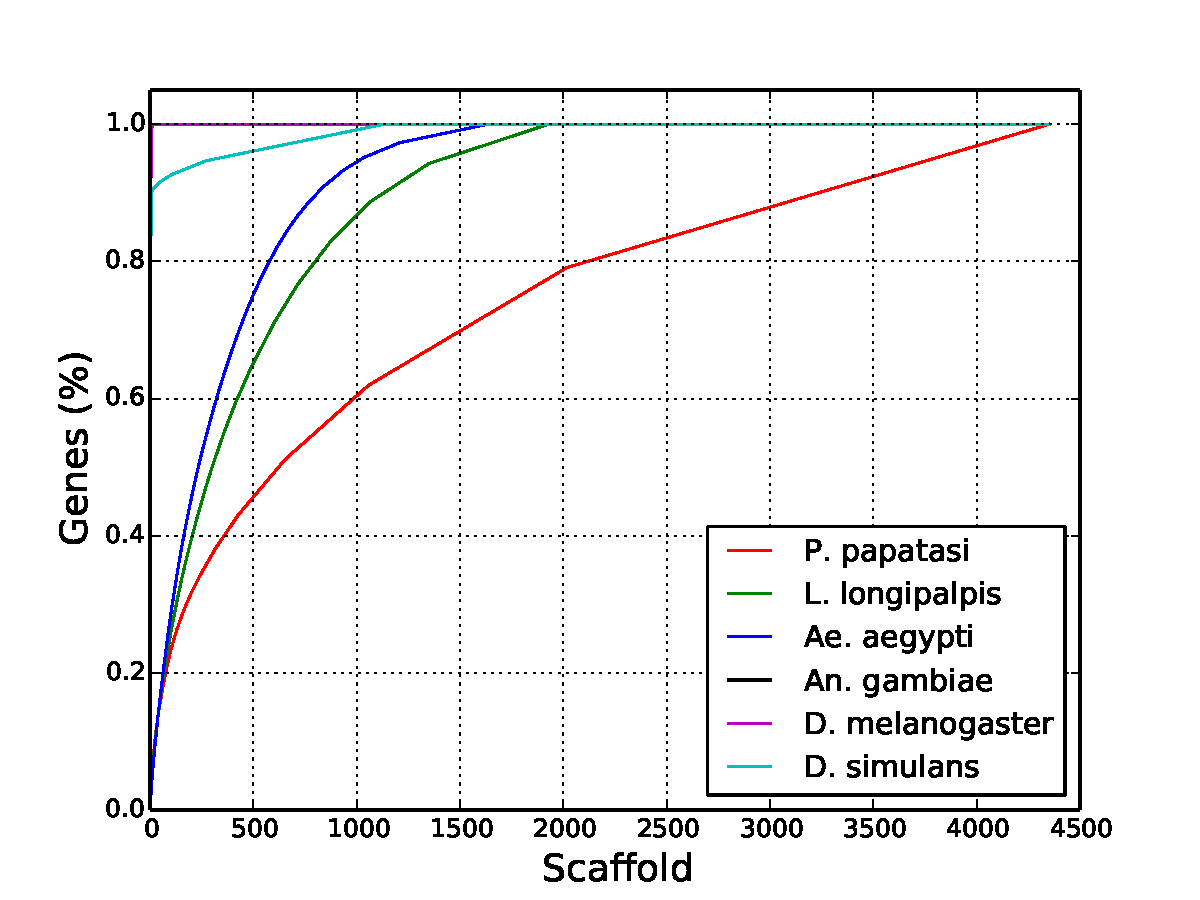
\includegraphics[width=\textwidth]{figures/synteny/gene_scaffold_cdf.pdf}
    \caption{Scaffold Genes CDF}
  \end{subfigure}
  \label{fig:scaffolds}
  \caption{}
\end{figure}

\subsubsection{Analysis of Macrosynteny}
Qualitative comparison of the \emph{L. longipalpis} and \emph{P. papatasi} genomes does not indicate the presence of macrosynteny (Figure~\ref{fig:synteny-dotplots-sandflies}).  Similarly, comparison of the \emph{Ae. aegypti} and \emph{A. gambiae} genomes also fail to demonstrate the presence of synteny (Figure~\ref{fig:synteny-dotplots-mosquitoes}).

In contrast, comparison of the \emph{D. melanogaster} and \emph{D. simulans} genomes indicates extensive presence of synteny (Figure~\ref{fig:synteny-dotplots-drosophila}).  Comparison of the \emph{A. gambiae} and \emph{D. melanogaster} genomes suggest some evidence of synteny but qualitative analysis alone is not sufficient to make a determination (Figure~\ref{fig:synteny-dotplots-anopheles-drosophila}).


\begin{figure}[H]
  \centering
  \begin{subfigure}[b]{0.45\textwidth}
    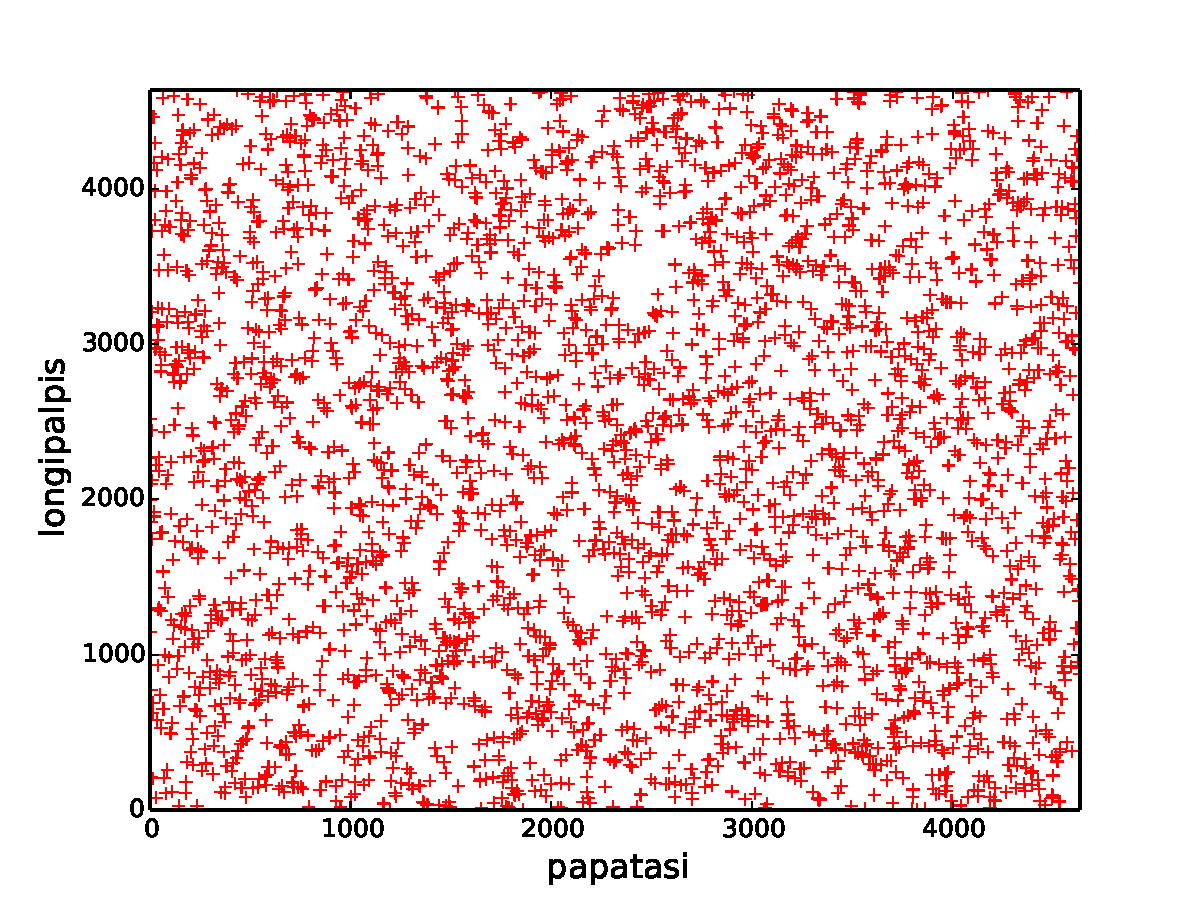
\includegraphics[width=\textwidth]{figures/synteny/papatasi_longipalpis_plot}
    \caption{\emph{L. longipalpis} vs. \emph{P. papatasi}}
    \label{fig:synteny-dotplots-sandflies}
  \end{subfigure}
  ~
  \begin{subfigure}[b]{0.45\textwidth}
    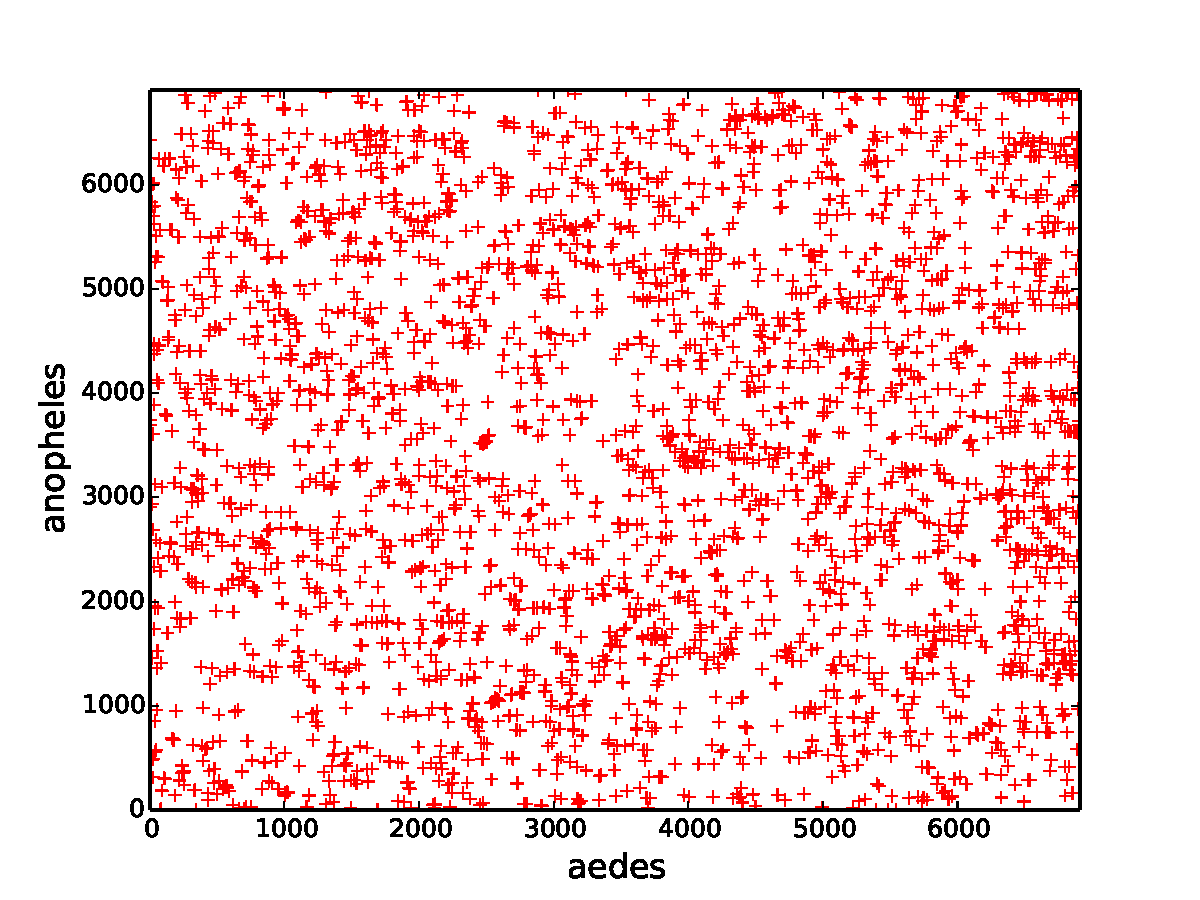
\includegraphics[width=\textwidth]{figures/synteny/aedes_anopheles_plot}
    \caption{\emph{Ae. aegypti} vs. \emph{A. gambiae}}
    \label{fig:synteny-dotplots-mosquitoes}
  \end{subfigure}
  ~
  \begin{subfigure}[b]{0.45\textwidth}
    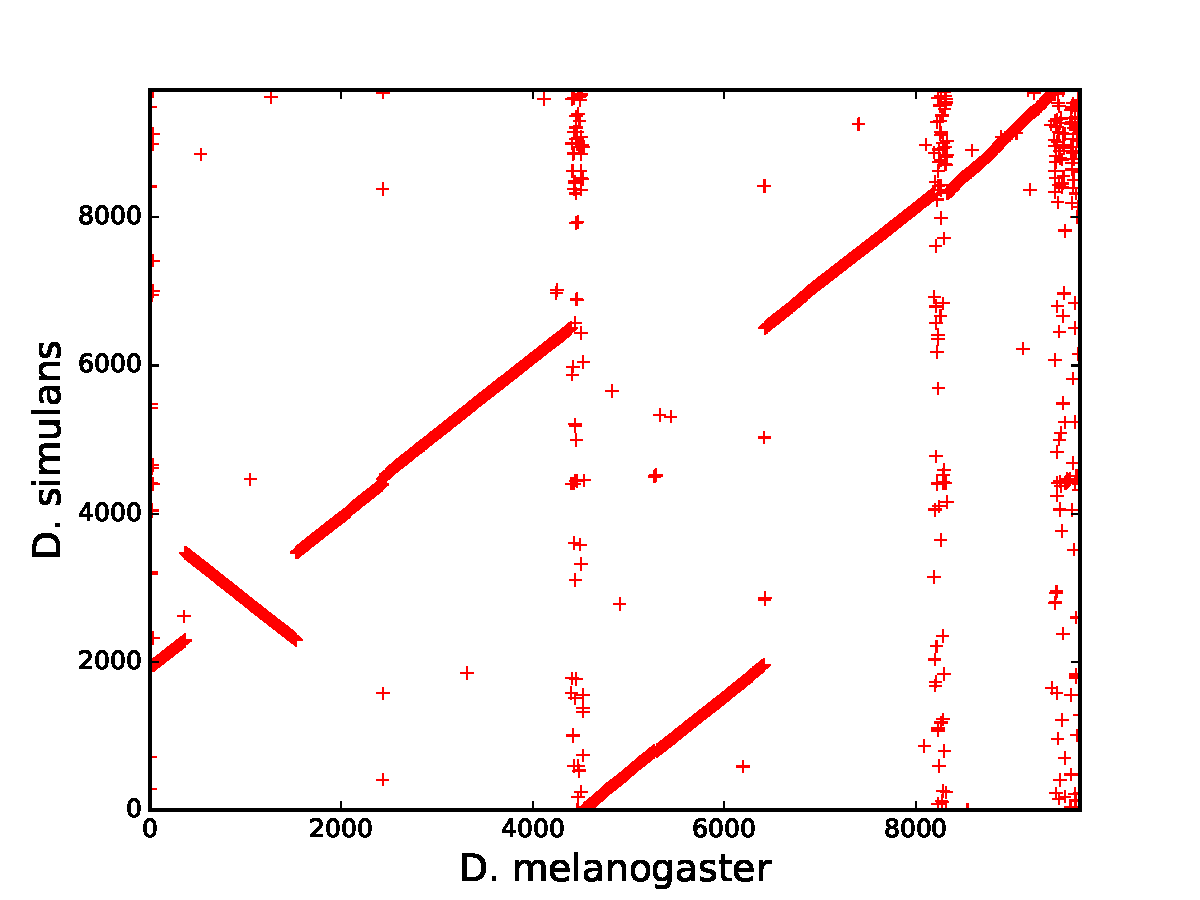
\includegraphics[width=\textwidth]{figures/synteny/dmel_dsim_plot}
    \caption{\emph{D. melanogaster} vs. \emph{D. simulans}}
    \label{fig:synteny-dotplots-drosophila}
  \end{subfigure}
  ~
  \begin{subfigure}[b]{0.45\textwidth}
    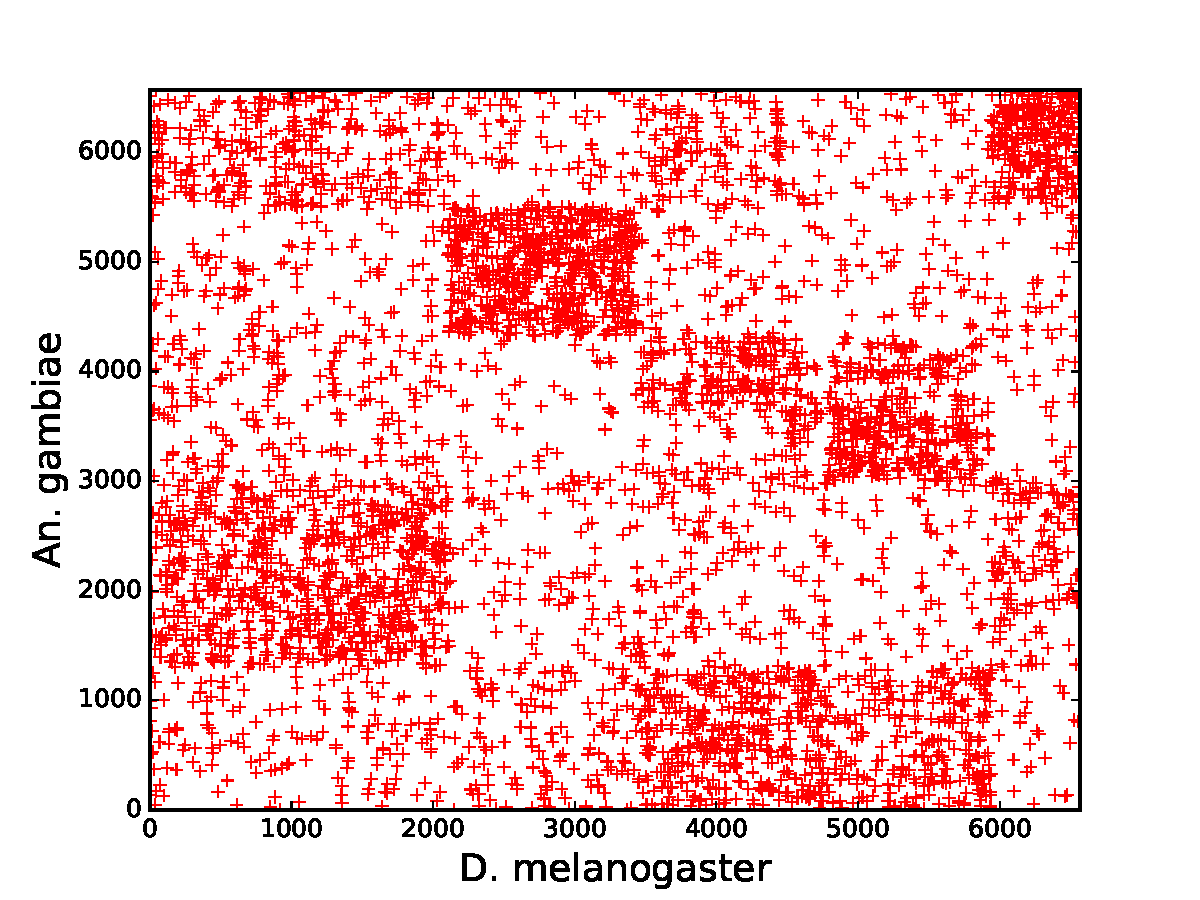
\includegraphics[width=\textwidth]{figures/synteny/dmel_anopheles_plot}
    \caption{\emph{A. gambiae} vs. \emph{D. melanogaster}}
    \label{fig:synteny-dotplots-anopheles-drosophila}
  \end{subfigure}
\label{fig:dot-plots}
\caption{Qualitative Analysis of Synteny}
\end{figure}

\textcolor{red}{TODO Muller elements}

\subsubsection{Analysis of Microsynteny}

\begin{figure}[H]
  \centering
  \begin{subfigure}[b]{0.45\textwidth}
    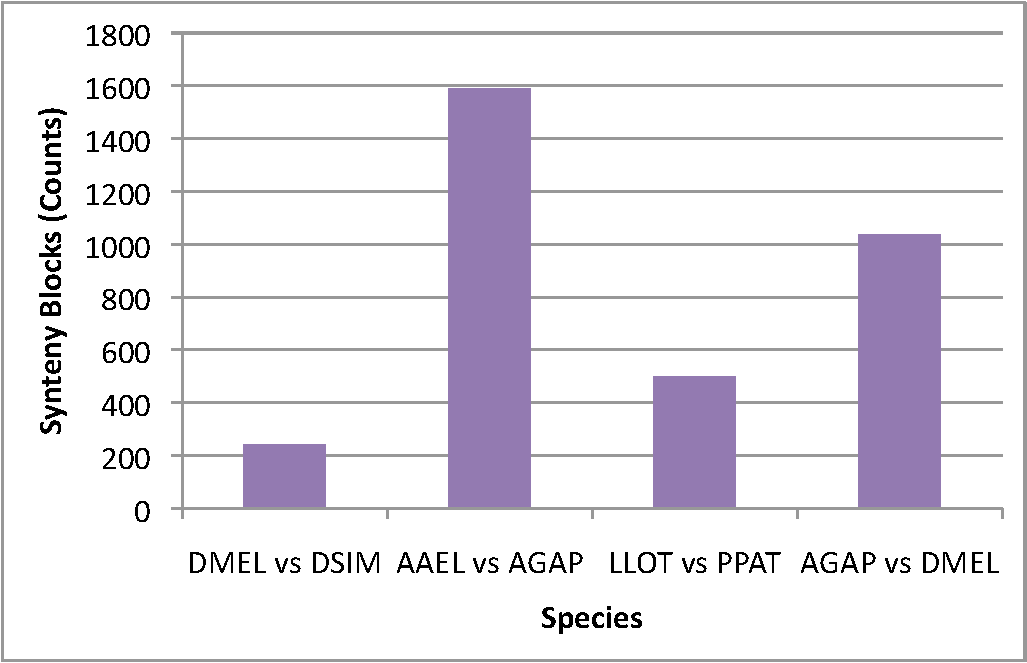
\includegraphics[width=\textwidth]{figures/synteny/block_counts}
    \caption{Number of Synteny Blocks}
    \label{fig:synteny-dist-counts}
  \end{subfigure}
  ~
  \begin{subfigure}[b]{0.45\textwidth}
    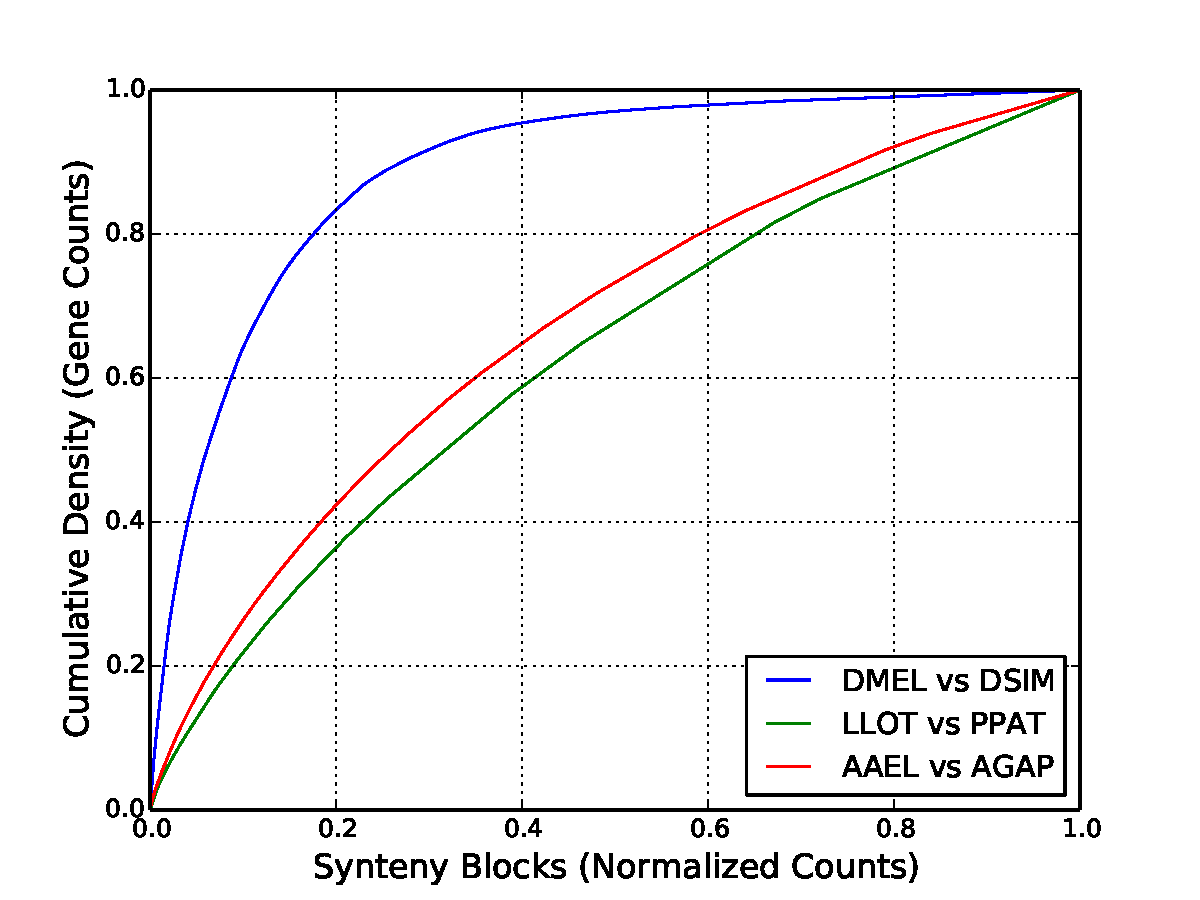
\includegraphics[width=\textwidth]{figures/synteny/sandflies_mosquitoes_drosophila_orth_cdf}
    \caption{Cumulative Density of Synteny Block Sizes}
    \label{fig:synteny-dist-cdf}
  \end{subfigure}
\label{fig:synteny-dist}
\caption{Quantitative Analysis of Synteny}
\end{figure}

\textcolor{red}{analysis of individual blocks}

\subsubsection{Annotation of \emph{L. longipalpis} vs. \emph{P. papatasi} Microsynteny Blocks}

\subsection{Discussion and Conclusion}
\pagebreak
\section{RNASeq}

\subsection{Introduction}

\subsection{Methods}

\subsubsection{\emph{De novo} Assembly with Trinity}

\subsubsection{GO Term Distributions}

\begin{figure}[H]
  \centering
  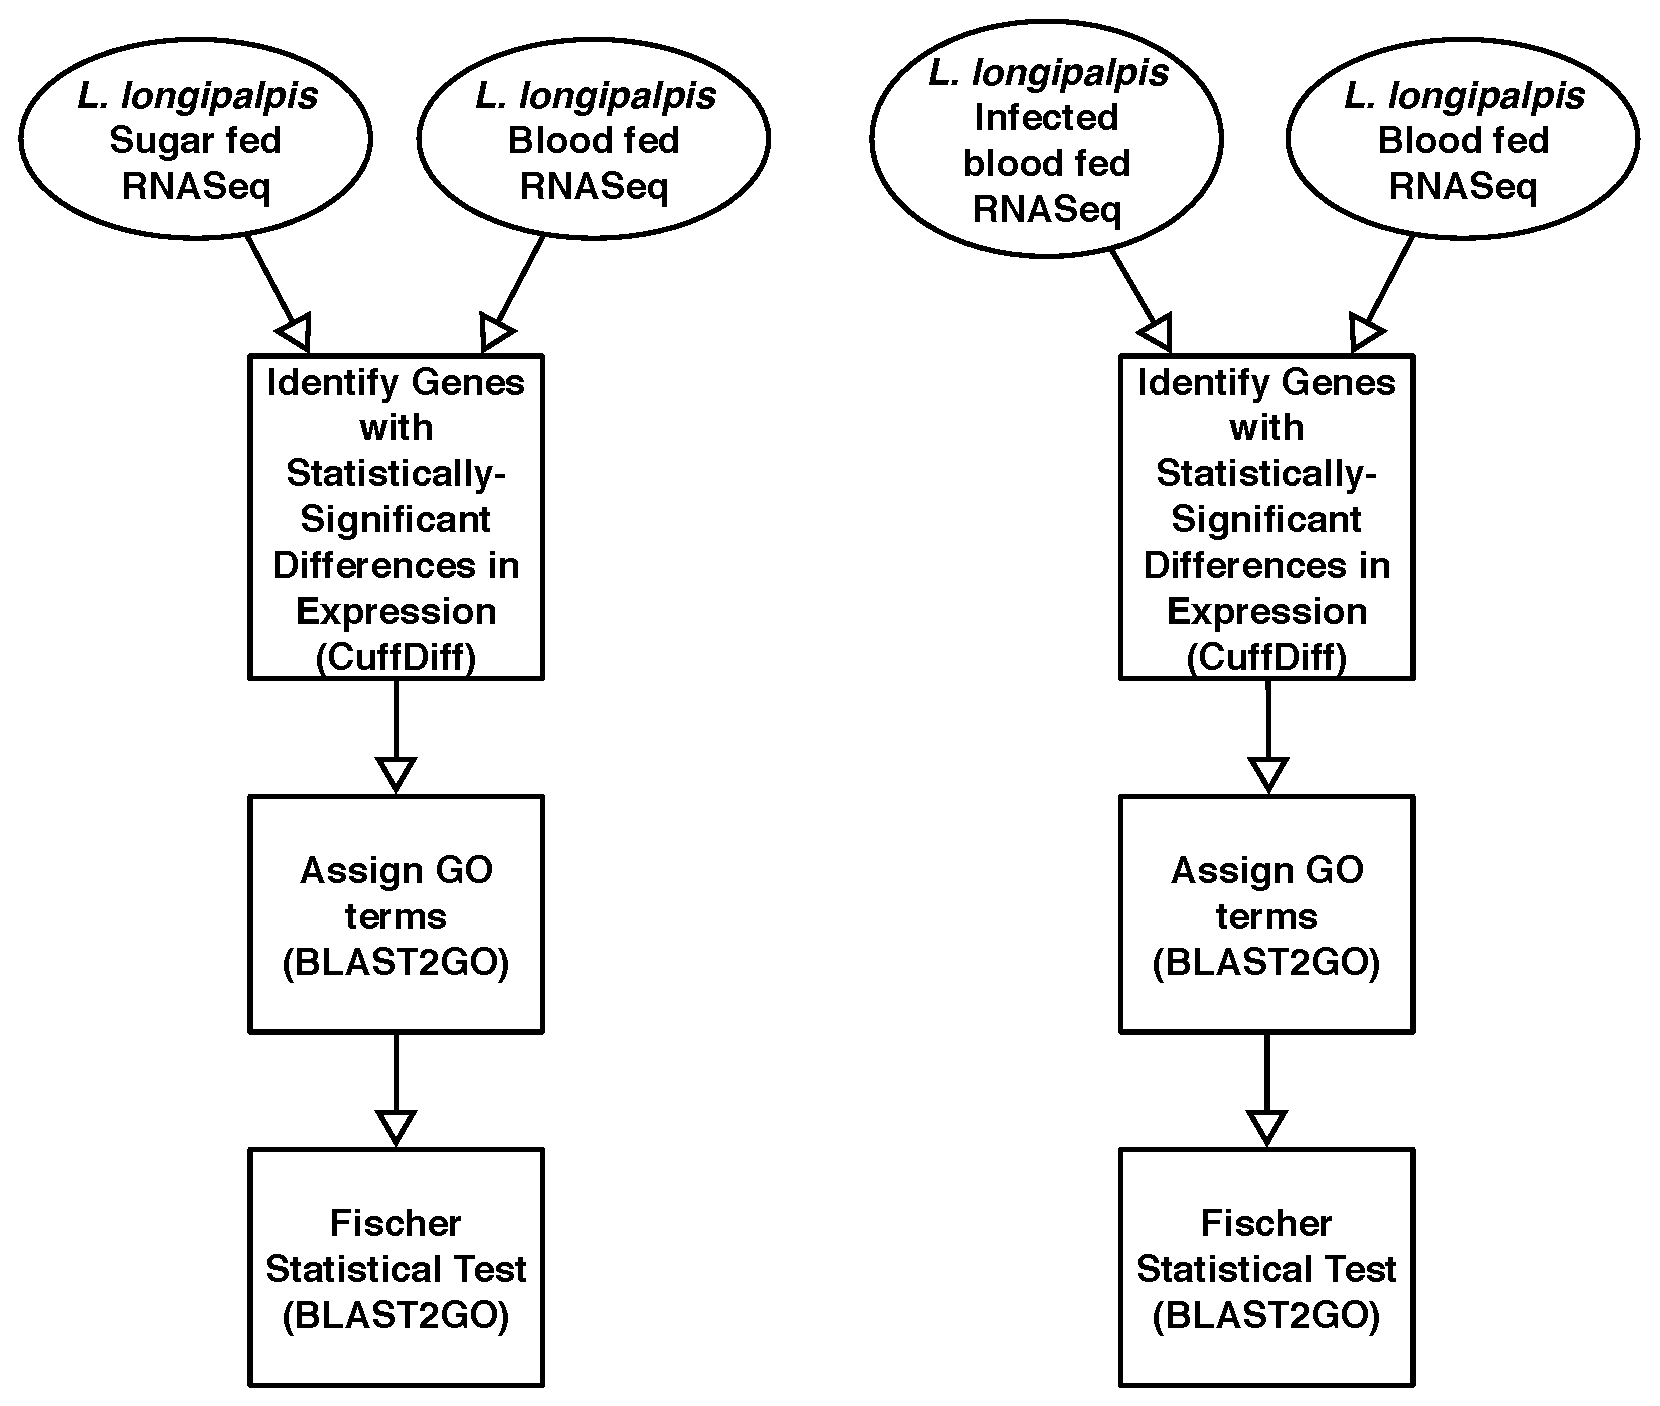
\includegraphics[width=0.7\textwidth]{figures/rnaseq/cuffdiff_workflow}
  \caption{Workflow for Comparing Gene Expression}
  \label{fig:rnaseq-cuffdiff-workflow}
\end{figure}

\subsection{Results}

\subsubsection{Analysis of RNASeq Assemblies}

\subsubsection{GO Term Distribution Differences}

\begin{table}[H]
  \centering
  \begin{tabular}{c c c} \hline
  \emph{Time Point} & \emph{Blood Fed vs Sugar Fed} & \emph{Infected Blood Fed vs Blood Fed} \\ \hline
  6H & 3,111 & 271 \\ \hline
  24H & 4,120 & 658 \\ \hline
  144H & 4,571 & 290 \\ \hline
  \end{tabular}
  \caption{Number of Genes with Statistically-Significant Differential Expression}
  \label{tab:stat-sig-genes}
\end{table}

\subsubsection{Pathway Analysis}

\subsubsection{Differential Expression by Gene Family}


\subsection{Discussion and Conclusion}
\pagebreak
\section{Project TBD}

\subsection{Introduction}

\subsection{Methods}

\subsection{Results}

\subsection{Discussion and Conclusion}
\pagebreak
\chapter{\uppercase{Conclusion}}

\pagebreak

\appendix
\section{A Domain-Driven, Generative Data Model for BigPetStore}

\subsection{Abstract}
Generating large amounts of semantically-rich data for testing big data workflows is paramount for scalable performance benchmarking and quality assurance in modern machine-learning and analytics workloads.  The most obvious use case for such a generative algorithm is in conjunction with a big data application blueprint, which can be used by developers (to test their emerging big data solutions) as well as end users (as a starting point for validating infrastructure installations, building novel applications, and learning analytics methods).

We present a new domain-driven, generative data model for BigPetStore, a big data application blueprint for the Hadoop ecosystem included in the Apache BigTop distribution. We describe the model and demonstrate its ability to generate semantically-rich data at variable scale ranging from a single machine to a large cluster.  We validate the model by using the generated data to answer questions about customer locations and purchasing habits for a fictional targeted advertising campaign, a common business use case.

\subsection{Introduction}
Big data applications process large, dynamic, multidimensional data sets with the general goal of information and knowledge extraction.  With the wide variety of big data tools available and lagging documentation, both developers and users of big data systems benefit from the availability of realistic example applications.  For developers, such applications are useful for testing, benchmarking, and evaluating design choices; for users, example applications provide starting points for learning methods, developing their own applications, and implementing new analytics workflows.

BigPetStore is one such big data application blueprint built around processing transaction data for a fictional chain of pet stores.  BigPetStore targets the Hadoop \cite{Hadoop} ecosystem with examples implemented for loading, cleaning, aggregating, and performing analytics on data using Hive \cite{Thusoo2010}, Pig \cite{Olston2008,Gates2009}, and Mahout \cite{Mahout}. BigPetStore has been incorporated into the open-source Apache BigTop distribution \cite{BigTop}, where it is used for testing and as a reference application. One of BigPetStore's key features is the ability to scale from a single machine to a large cluster, making it easy to develop projects on a local machine and transfer the application to a large cluster for production testing.

To achieve the project's goals of providing high-quality, realistic examples, BigPetStore requires semantically-rich, complex data. At its core, BigPetStore relies on a generative data model for producing synthetic transaction data. Despite the growing number of real data sets now publically available, synthetic data generators have a number of advantages for BigPetStore over real data sets. The synthetic data generator can be packaged with BigPetStore, avoiding the cost, time, and infrastructure needed to host, transfer, and store large data sets. Synthetic data generators are scalable, allowing the user to choose how much data to generate -- a requirement for supporting BigPetStore's goal of running on both single machines and large clusters.  Licensing and privacy issues are avoided with the use of synthetic data sets. And lastly, the generated data can be customized by the user, allowing the user to generate data with specific criteria amenable to testing.  For example, a user may generate transactions from a small number of purchasable items so that clustering results can be easily visualized.

A variety of approaches for generating synthetic data sets exist.  TeraGen and the Intel Hadoop Benchmark Suite \cite{Huang2010} are popular tools that can generate data sets quickly and at any scale, but the resulting data is semantically-void and not useful for much more than simple benchmarks.  Multiple frameworks exist for generating synthetic data sets that satisfy relational database schemas \cite{Ghazal2013,Rabl2011a,Frank2012,Rabl2011,Gray1994,Bruno2005,Hoag2007}, and several approaches even provide domain-specific languages \cite{LogSynth,Bruno2005,Hoag2007} for specifying additional constraints (such as which distributions to sample from and allow for modeling basic relationships between fields using simple arithmetic equations \cite{Alexandrov2012}).

Recent work has addressed some aspects of the need for more dynamic data set generation: Arasu, et al. \cite{Arasu2011} demonstrated that constraint-solving techniques could be used as an alternative to procedural approaches. Such frameworks allow for reproducing the structural properties of real data, but the frameworks are not expressive enough to describe the dynamic generation processes and latent variables that would be needed to embed the desired informational complexity and rich semantics needed for BigPetStore's analytics examples.

Realizing the difficulty in creating a generic framework capable of modeling the semantics of real data, recent work\cite{Alexandrov2013} has focused on generating synthetic data sets that satisfy characteristics learned from real reference data. Such approaches appear promising but will need to overcome the difficulties of accurately training models, especially on raw data instead of features.

Until such purely generic methods reach maturity, BigPetStore's needs are best met by a customized, domain-driven model. Another example of such a model is The Information Discovery and Analysis System (IDAS) Data Set Generator (IDSG) \cite{Jeske2005,Lin2006}. IDSG was developed to test the effectiveness of IDASs in identifying potential terrorism threat scenarios using synthetic data.  Like BigPetStore, the developers of IDSG needed to avoid licensing restrictions and privacy issues associated with real data.

BigPetStore's current model has been used successfully to generate terabytes of synthetic data and is used regularly for testing in Apache BigTop, showcasing the value of the approach.  The current model is limited, however, in its ability to generate data that is semantically rich, limiting progress on BigPetStore's goals of providing realistic analytics examples.

In this work, we present a new domain-driven model and simulation method for BigPetStore.  Compared with BigPetStore's previous data generator, our model and implementation can generate data which contains geospatial, temporal, and quantitative features, similar to the type of data which businesses and organizations might typically encounter.  Combining the features of the TeraGen (scalability)  and MovieLens \cite{MovieLens} (semantically rich) input data sets commonly used for big data benchmarking, we present a synthetic data set generator which can be used to benchmark lower level tasks (such as sorting) as well as higher level tasks (such as clustering, recommending, and search indexing) at arbitrary scale.  To demonstrate that the model generates data with desirable properties, we performed an example analysis designed to guide a fictional advertising campaign (a typical business use case). The model's implementation was made available as open source software.

\subsection{Overview of Model \& Simulation Procedures}
Our generative model combines various well-known mathematical modeling techniques to simulate the factors affecting customers' purchasing habits.  Each part of the model is derived from \emph{ab initio} assumptions.  In several cases, real data is used to parameterize parts of the model. 

\subsubsection{Description of Generated Data}
The model generates data for four types of records: stores, customers, transactions, and transaction items (Figure~\ref{fig:relational-data-model}).  Store records contain both a unique identifier and a location in the form of a 5-digit zip code. Customer records consist of a unique identifier, a name, and a location given as a 5-digit zip code. Transaction records consist of a transaction identifier, a customer identifier, a store identifier, and a time given in days since the beginning of the simulation. Transaction item records contain a transaction identifier and an item description.  The item description is a list of key-value pairs stored as a string.  Key-value pairs are used since item characteristics differ depending on the type of item.  For example, dog food has a brand, a flavor, a size (in lbs), and a per-unit cost, while poop bags have a brand, a color, a count, and a per-unit cost.

\begin{figure}[!t]
  \centering
  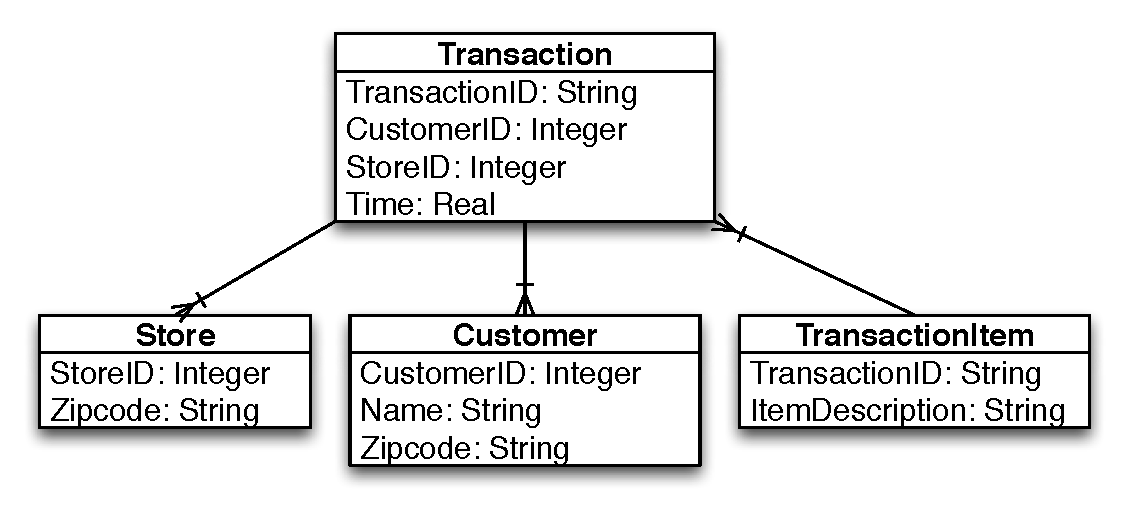
\includegraphics[width=3.5in]{figures/bigpetstore/transactions_data_model.eps}
  \caption{Relational Data Model for Generated Data}
  \label{fig:relational-data-model}
\end{figure}

\subsubsection{Generation of Stores}
The locations of the stores are modeled by a probability density function (PDF) that gives the probability that a store's location is the given zip code. We designed the PDF to give to zip codes in high-population, high-income areas the highest probabilities. The PDF is composed of two individual PDFs. One PDF determines the probability of each zip code as the population of that zip code over the total population:

\begin{equation*}
p(\text{location}=z | \text{population}(z)) = \frac{\text{population}(z)}{\sum_{i} \text{population}(i)}
\end{equation*}

The second PDF scales the probabilities of the zip codes by their incomes.  The zip code with the highest-income has a probability $s$-times larger than that of the lowest-income zip code. The values in-between are interpolated using an exponential function:

\begin{equation*}
p(\text{location}=z | \text{income}(z)) = s ^ {\big( \frac{\text{income} - \min_i{\textrm{income}(i)}} {\max_i{\textrm{income}(i)} - \min_i{\textrm{income}(i)}} - 1 \big)}
\end{equation*}

The combined PDF is given as: 

\begin{align*}
p(\text{location}=z) = &Z p(\text{location}=z | \text{population}(z)) \\
&p(\text{location}=z | \text{income}(z))
\end{align*}

where $Z$ is the normalization factor.  Given the small size ($\approx$30,000 zip codes) of the data set, $Z$ can be found directly by iterating over all of the zip codes and summing the scores. The population and household income data for the zip codes were taken from from the U.S. Census American Community Survey \cite{ACS}.  The stores' locations are generated by sampling zip codes from the PDF.

\subsubsection{Generation of Customers}
For each proposed customer location zip code $z$, we compute the distance $d_m(z)$ between $z$ and each store's zip code $s_z$ to find the closest store.  The zip codes' latitudes and longitudes (taken from the Zip Code Database Project \cite{Zips}) are used to compute the distances. Each zip code $z$ is assigned a weight $w_z$ according to its distance $d_m(z)$ to the nearest store using an exponential distribution with the average distance $\beta$:

\begin{align*}
&w_z = \beta^{-1} \exp(-\beta^{-1} \, d_m(z)) \\
&d_m(z) = \min_{s_z} \, d(z, s_z)
\end{align*}

The customer's zip code is chosen by sampling from the zip codes with the probabiltiy of choosing each zip code $z$ proportional to its weight $w_z$.

Names are generated using data from the Name Database\cite{NameDB}. Each record in the database gives a name, a weight, and flag indicatings if the name can be used as a first name, a last name, or both.  PDFs generated for the first and last names using the weights.  The customer's name is generated by sampling a first name and a last name from each PDF respectively.

We determine the number of pets $N_p$ each customer has by sampling from a discrete uniform distribution of integers. We then sample the number of dogs $N_d$ as a discrete uniform distribution of integers between 0 and $N_p$.  The remaining number of pets are assigned to be cats.

\begin{align*}
N_c = N_p - N_d \\
N_d \sim U(0, N_p) \\
N_p \sim U(1, b)
\end{align*}

\subsubsection{Simulation of Transactions}
A transaction simulation is run for each customer. The transaction's store is set to the store located closest to the customer.  Transaction times are generated from a Monte Carlo process that proposes transaction times based on the usage of the customer's items and Poisson processes modeling the amount of time between the customer visiting the store and running out of the items (Section~\ref{sec:transaction-times}).  The purchased items are generated by a Hidden Markov Model (HMM) parameterized by the transaction time and amount of time remaining for the items in the customer's inventory (Section~\ref{sec:transaction-purchases}).

\begin{figure}[!t]
  \centering
  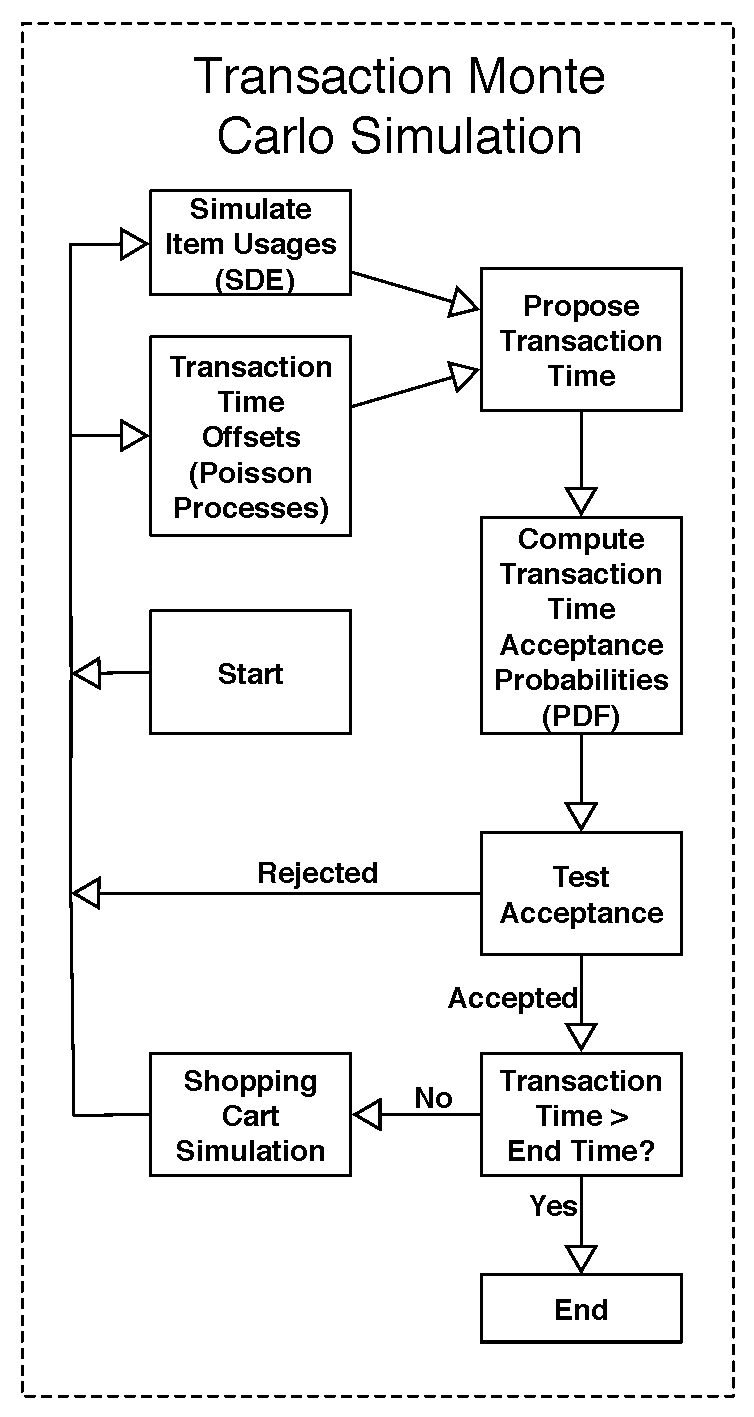
\includegraphics[width=3.5in]{figures/bigpetstore/transaction_simulation.eps}
  \caption{Flowchart of Transaction Monte Carlo Simulation}
  \label{fig:trans_sim}
\end{figure}

\subsubsection{Simulation of Transaction Times} \label{sec:transaction-times}
Transaction times are simulated using a Monte Carlo method (Figure~\ref{fig:trans_sim}).  The usage over time of each item category is simulated. Items categories are groups of items which are interchangeable such as ``dry dog food,'' ``dry cat food,'' and ``kitty litter.'' The time between the customer's visit to the store to buy more items in each category and the exhaustion time of that item category is modeled using a Poisson process. Proposed transaction times for each item category are computed based on the exhaustion time and time sampled from the Poisson process. The earliest transaction time is taken as the overall proposed transaction time.  The probability of the transaction time is calculated using a PDF.  If rejected, new transaction times are proposed.  Otherwise, the purchased items are modeled using a separate process (discussed below). After the items are chosen, the process begins again with the simulation of the item category usages.

In the first stage of the process, the usage of items over time is modeled using a stochastic differential equation (SDE):

\begin{equation*}
\frac{da_i}{dt} = \min \{-\mu_i + \sigma_i\, dW_i(t), 0\}
\end{equation*}

where $a_i$ is the amount of item category $i$ ``stuff'' remaining at time $t$. The variable $\mu_i$ gives the average usage rate and $\sigma^2_i$ gives the variance of the usage rate for item category $i$. The SDE is numerically integrated using the Euler-Maruyama method\cite{Klouden13} with time step $\Delta t_n$ sampled from an exponential distribution:

\begin{align*}
&a_{n+1, i} = a_{n,i} - \min \{\mu_{i, c} \, \Delta t_n + \sigma_{i, c} \, \sqrt{\Delta t_n} R_n, 0.0\} \\
&t_{n+1} = t_n + \Delta t_n \\
&\Delta t_n \sim \text{Exp}(\beta^{-1}_{i,c}) \\
&R_n \sim \text{N}(0, 1)
\end{align*}

where $a_{n, i}$ is the amount remaining of item category $i$ at time step $t_n$, $\mu_{i,c}$ is the average amount used per time used, $\sigma^2_{i,c}$ is the variance of the amount used per time used, and $\beta_{i,c}$ is the item category's average amount of time between uses for customer $c$.  The parameters $\mu_{i, c}$, and $\sigma^2_{i,c}$ are computed from a base rate for each item category multiplied by the number of pets of the appropriate species the customer $c$ has.  The exhaustion time $T_{E,i}$ for each item category is found by simulating the usage until $a_{n,i} \leq 0$.

The proposed transaction time is found from the exhaustion times (Eq.~\ref{eq:transaction-times}).  For each item category, the offset time $T_{O, i}$ between when a customer would visit the store and the exhaustion time is sampled from an exponential distribution. The distribution is parameterized by $\beta_c$, the average number of days before triggering a transaction. The parameter $\beta_c$ is set separately for each customer $c$ by sampling from a uniform distribution. A proposed transaction time $T_{P, i}$ for each item category is found by subtracting the offset time $T_{O, i}$ from the exhaustion time $T_{E, i}$.  The earliest proposed transaction time is taken as the overall proposed transaction time $T_T$.

\begin{align} \label{eq:transaction-times}
&T_T = \min_i \, \{  T_{P, i}\} \\
&T_{P, i} = T_{E,i} - T_{O, i} \nonumber\\
&T_{O, i} \sim \text{Exp}(\beta^{-1}_c) \nonumber \\
&\beta_c \sim \text{U}(a, b) \nonumber
\end{align}

The acceptance probability $p(t_{n+1}=T_T|t_n)$ of the proposed transaction time $T_T$ is modeled using a PDF (Eq.~\ref{eq:transaction_time_pdf}). For now, the PDF only ensures that the proposed transaction time is more recent than the last transaction time.

%The PDF could be extended to incorporate additional factors including time-dependent events such as sales, weather, and the amount of money the customer has available at the time.

\begin{equation} \label{eq:transaction_time_pdf}
p(t_{n+1}=T_T|t_n) = \left\{ 
  \begin{array}{l l}
   1 & \quad t_{n+1} \geq t_n\\
   0 & \quad t_{n+1} < t_n
  \end{array} \right.
\end{equation}

The proposed transaction time is accepted if $p(t_{n+1}=T_T) < r$, where $r \sim \text{U}(0, 1)$. Until the proposed transaction time is accepted, a new proposed transaction time is generated by sampling new offset times. If the proposed transaction time is accepted, the purchased items are chosen through a separate simulation discussed in Section~\ref{sec:transaction-purchases} below. Transactions are generated until the accepted transaction time is later than the end time given as a simulation parameter.

\begin{figure*}[!t]
  \centering
  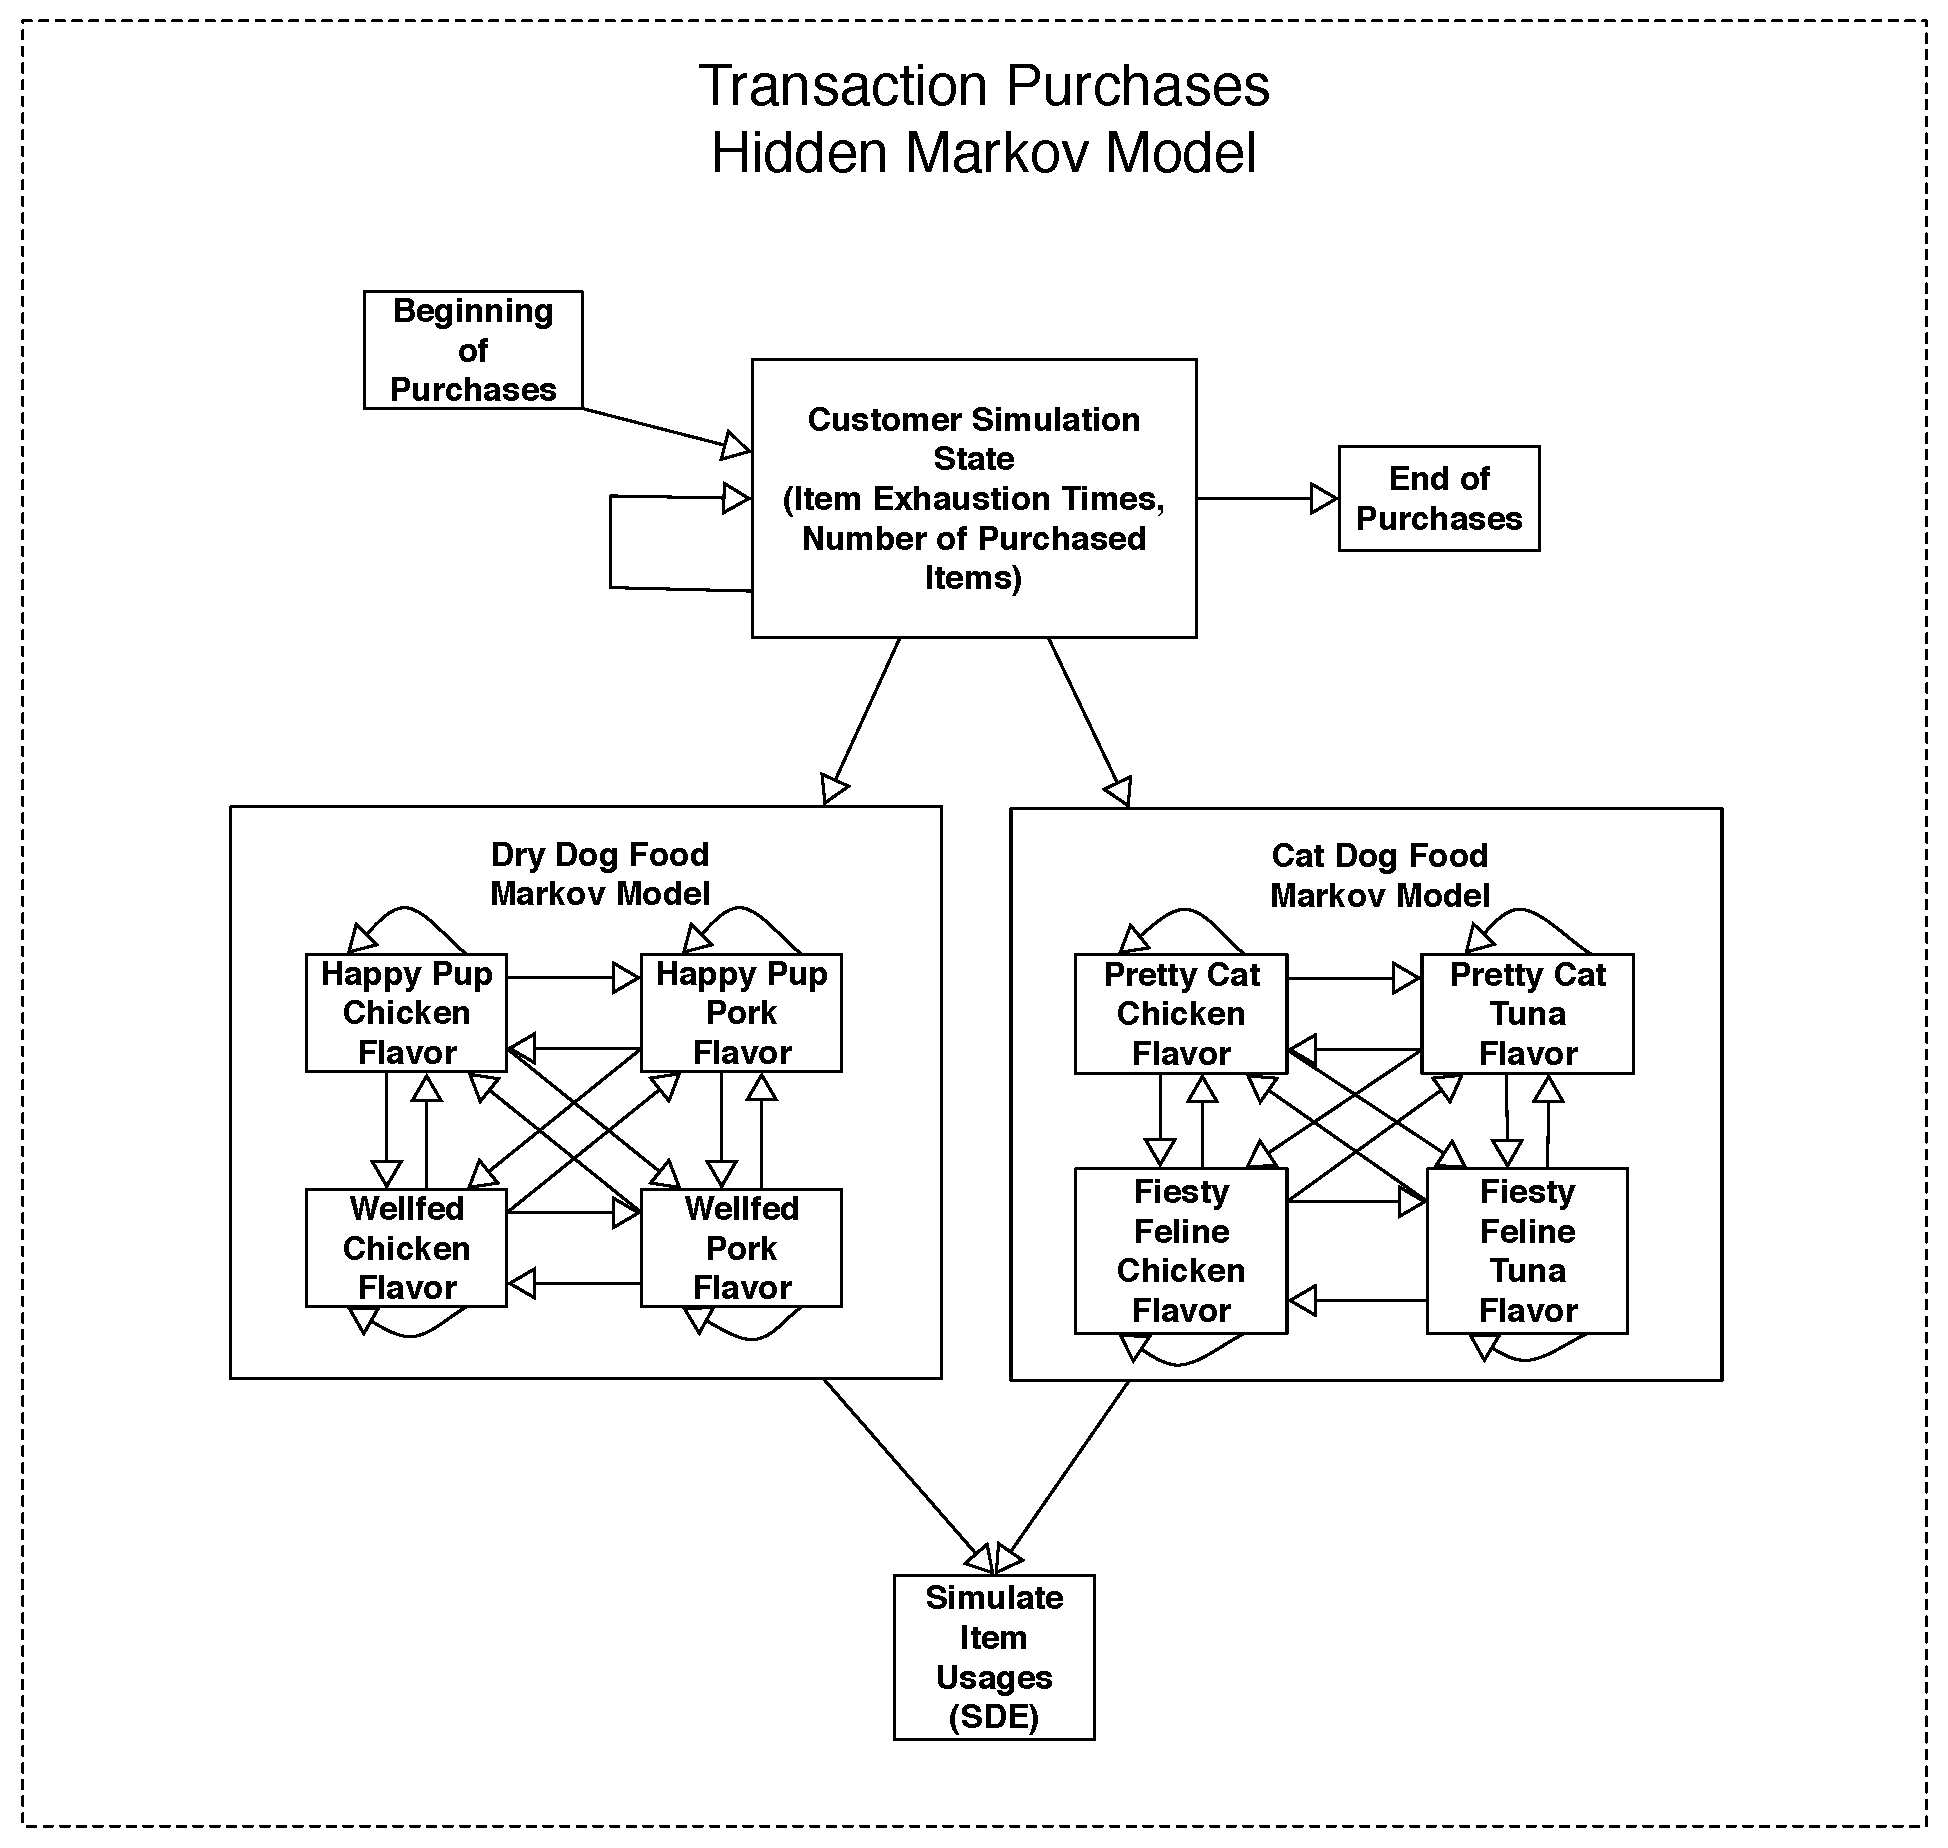
\includegraphics[width=6in]{figures/bigpetstore/shopping_cart_simulation.eps}
  \caption{Example Shopping Cart Hidden Markov Model}
  \label{fig:shopping_cart_sim}
\end{figure*}

\subsubsection{Simulation of Transaction Items} \label{sec:transaction-purchases}

A customer's purchases in each transaction are modeled using a layered Hidden Markov Model (HMM) (Figure~\ref{fig:shopping_cart_sim}).  The HMM has three types of states: the start state, the purchase states, and the stop state. There are an infinite number of purchase states, parameterized by the exhaustion times of the customer's item categories and the transaction time.

The observables of the states correspond to the item categories.  Each item category $i$ is assigned a weight $w_i$ according to the amount of time between the transaction time $T_t$ and $T_{E,i}$ when each item category will be exhausted (based on the usage simulations):

\begin{align} \label{eq:category-weights}
&w_i = - \beta^{-1}_c \exp(-\beta^{-1}_c (T_{E, i}- T_T)) \\
&\beta^{-1}_c \sim U(a,b) \nonumber
\end{align}

where $\beta_c$ the average number of days between when a customer purchases an item and the exhaustion time. The value $\beta_c$ is set separately for each customer by sampling from a uniform distribution. The value $w_i$ is used to model the propensity for a customer to purchase an item they will run out at time $T_{E, i}$ in the future when at the store at time $T_T$.

The item category is chosen by sampling from the item categories with the probability of choosing each item category $i$ proportional to its weight $w_i$.

Markov Models are used to model the customer's purchasing behavior for each item category.  Each state $X_n$ corresponds to an item in that category. The customer's buying habits are determined by the transition probabilities:  

\begin{align}
Pr(X_{n+1}&=x|X_n=y) = \nonumber \\
& \left\{ 
  \begin{array}{l l}
   (1.0 - p_l) \, Pr(x,y)  & \quad \text{if $x \neq y$}\\
   p_l & \quad \text{if $x = y$}
  \end{array} \right.
\end{align}

where $w_l$ is the loopback probability, giving the probability of choosing the same item $y$ again. The function $Pr(x,y)$ gives the probability of choosing the item $x$ given that the previous item was $y$:

\begin{equation*}
Pr(x,y) = \frac{\sum_f w_f w_{f,s}(x, y)}{\sum_{j \neq x} \sum_f w_f w_{f,s}(x, j)}
\end{equation*}

where $w_f$ is the weight of a particular field $f$.   The pair of items $x$ and $y$ are weighted  according to the equality of the values for each field:

\begin{equation*}
w_{f,s}(x,y) = \left\{ 
  \begin{array}{l l}
   w_{f,s}  & \quad \text{if $x$.$f$ = $y$.$f$}\\
   1 - w_{f, s} & \quad \text{if $x$.$f$ $\neq$ $y$.$f$}
  \end{array} \right.
\end{equation*} 

The weights $w_l$, $w_f$, and $w_{f, s}$ are chosen randomly for each customer:

\begin{align*}
&w_l \sim N(\mu, \sigma^2) \\
&w_f \sim N(\mu, \sigma^2) \\
&w_{f, s} \sim N(\mu, \sigma^2)
\end{align*}

If the weights are greater than 1, they are rounded down to 1.  Likewise, if the weights are less than 0, they are rounded up to 0.

To simulate an item purchase, the chosen Markov model is transitioned forward by one state. The current states of the Markov models are kept between purchases.  After an item is chosen, the item category's exhaustion time is updated by propagating the item category usage SDE described in Section~\ref{sec:transaction-times}, resulting in an implicit creation of the next possible purchase state in the HMM.

After each purchase, the HMM's current state is transitioned to either the new purchase state or the stop state.  The probability of choosing the next state is 

\begin{align*}
&Pr(X_{n+1}=\text{stop}|X_n) = p(\text{stop})\\
&Pr(X_{n+1}=\text{purchase}|X_n) = 1 - p(\text{stop})
\end{align*}

where $p(\text{stop})$ is the probability of choosing the stop state and is given by

\begin{equation*}
 p(\text{stop}) = \frac{w_{\text{stop}}}{w_{\text{stop}} + \sum_i w_i}
\end{equation*}

where $w_{\text{stop}}$ is the weight of the stop state and is a simulation parameter and the weight $w_i$ of each item category $i$ was given earlier in Eq.~\ref{eq:category-weights}.

If the stop state is chosen, the transaction is finished and the next transaction is started according to the procedure presented in Section~\ref{sec:transaction-times}.

%The HMM can be extended to consider additional factors such as the amount of money spent so far in the transaction and the customer's spending habits.

\subsection{Implementation}
The models and simulations were implemented using Python. The source code is available at \url{https://github.com/rnowling/bigpetstore-data-generator} under the Apache Public License v2.

\subsection{Evaluation of the Model}
In accordance with our original design goals, we evaluated the model and implementation in terms of their abilities to generate semantically-interesting data and scale from a single local machine to a cluster.

\subsubsection{Example Analysis of Generated Data}
To evaluate the semantic content of the generated data, we performed two example analyses in support of a fictional advertising campaign using data for 10 stores, 10,000 customers, and five years of transactions generated from the model. The analyses were designed to be realistic and driven by real-world business concerns.  Due to limited advertising budgets, businesses need to decide who to target and what sort of advertisements are likely to be effective for each type of customer.  We analyzed data generated from the model to determine where the advertising campaigns should be targeted geographically and identify customer purchasing profiles.

First, we wanted to identify how close most customers live to a store since advertising to people who live or work too far away from a store is unlikely to be effective and will increase our costs. We analyzed the distribution of distances between customers' homes and their nearest stores.  We found that most customers tend to live within 15 miles of their closest store, suggesting that we should limit our advertising to a 15-mile radius around each our store.

\begin{figure}[!t]
  \centering
  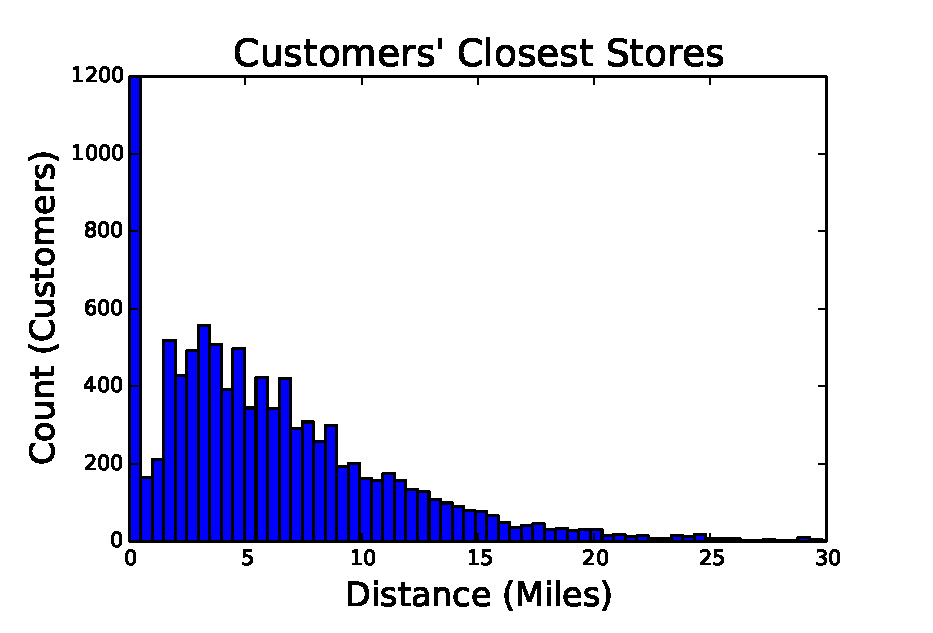
\includegraphics[width=3.5in]{figures/bigpetstore/customer_store_distances.eps}
  \caption{Distributions of Distances of Customers to Closest Stores}
  \label{fig:cluster_analysis}
\end{figure}

Secondly, we profiled our customers' purchasing habits to optimize the advertising campaign's effectiveness by customizing the advertised products for each customer.  For each customer, we generated a feature vector by computing the frequency with which they would purchase the same brand or flavor from one transaction to the next.  We clustered the customers' feature vectors using the KMeans algorithm with a range of cluster counts. Twenty clusters converged the error.

\begin{figure}[!t]
  \centering
  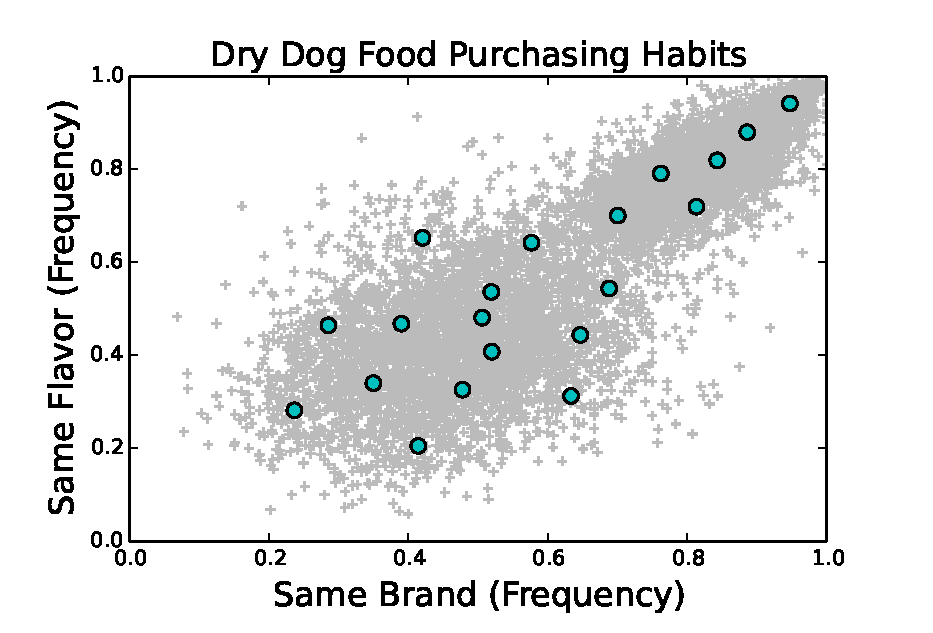
\includegraphics[width=3.5in]{figures/bigpetstore/cluster_analysis.eps}
  \caption{Clustering of Brand and Flavor Purchasing Preferences. Grey plus signs (+) represent customer data points, and cyan circles represent cluster centers.}
  \label{fig:cluster_analysis}
\end{figure}

Analysis of the feature vectors and clusters revealed four predominant purchasing profiles (Figure~\ref{fig:cluster_analysis}).  High frequencies of purchasing the same flavors repeatedly were tightly-correlated with high frequencies of purchasing the same brands -- these customers were likely to be happy with a particular item and kept purchasing the same item repeatedly.  For our advertising campaign, it would be unlikely to get these customers to purchase different items, so we should create incentives to purchase larger quantities, especially when inventory levels are high and needed to be depleted.  Other customers had a tendency to purchase either the same flavor or brand repeatedly, but varied in their choice of the other.  For customers who prefer a particular brand, we should target our advertising campaign to suggest other flavors sold by that brand.  Likewise, for customers who prefer a particular flavor, we should target our advertising campaign to suggest other brands with that flavor.  Lastly, some customers had very low frequencies of purchasing neither the same brand nor flavor.  Other factors, such as cost, not represented in this analysis may be driving these customers' purchasing habits and will need further study.


\subsubsection{Scaling of Data Size and Run Time}
BigPetStore aims to scale from a local desktop to a large cluster. To evaluate the scaling of the model and implementation, we benchmarked the data generator on a laptop with a 2 GHz Intel Core i7 CPU, 8 GB of RAM, and a 256 GB SSD using the Python implementation with a single thread. Using the test setup, between 1,500 and 2,000 transactions can be generated per second (Table~\ref{tab:benchmarks}). As the customers' transaction simulations are independent of one another, the transaction generation can easily be parallelized so that 1,500-2,000 transactions can be generated per thread per second.

\begin{table}[!t]
%% increase table row spacing, adjust to taste
\renewcommand{\arraystretch}{1.3}
% if using array.sty, it might be a good idea to tweak the value of
% \extrarowheight as needed to properly center the text within the cells
\caption{Benchmarks of Data Generator}
\label{tab:benchmarks}
\centering
%% Some packages, such as MDW tools, offer better commands for making tables
%% than the plain LaTeX2e tabular which is used here.
\begin{tabular}{|p{0.75cm}||p{1.2cm}||p{1cm}||p{1.25cm}||p{1cm}||p{1cm}|}
\hline
Stores & Customers & Simulated Time (years) & Transactions & Data Size (MB) & Run Time (min)\\ \hline
10 & 10,000 & 1 & 279,870 & 18 & 3.5 \\ \hline
%10 & 100,000 & 1 & 
100 & 10,000 & 1 & 279,586 & 18 & 3.5 \\ \hline
% 100 & 100,000 & 1 & 
10 & 1,000 & 5 & 123,309 & 8 & 1.1 \\ \hline
100 & 1,000 & 5 & 127,064 & 8 & 1.2 \\ \hline
10 & 10,000 & 5 & 1,275,542 & 84 & 11.0 \\ \hline
%10 & 100,000 & 5 & 
100 & 10,000 & 5 & 1,268,403 & 84 & 10.5 \\ \hline
\end{tabular}
\end{table}

The number of transactions (and hence, data size) grows as $O(N_c T)$ where $N_c$ is the number of customers and $T$ is the amount of time to be simulated. The amount of data generated can be scaled as large as necessary simply by increasing $N_c$ and $T$. Five years of transactions for 100,000 customers will generate approximately 1 GB of data. A terabyte of data can be generated by simulating 100 million customers over five years. 

\subsection{Discussion and Conclusion}
We have described a domain-driven mathematical model and accompanying simulation for generating semantically-rich data.  We validated the method by analyzing generated data to inform decisions in a fictional advertising campaign. Scalability testing combined with analysis of the implementation suggests that the data generation method can scale from small data sets appropriate for desktop development to large data sets for testing and benchmarking of clusters. We have released the implementation source code under the open-source Apache Public License v2.

We see many opportunities for building on the work presented.  We intend to expand the model to incorporate additional factors.  Deeper integration of existing fields such as location and purchasing profiles (e.g., to model regional purchasing preferences) will increase the variety of the semantic information encoded in the generated data. The incorporation of weather and climate data can be used to influence when customers shop, the types of products they buy, and the amount of products purchased. For example, customers would be less likely to shop during snow storms, more likely to buy items such as winter apparel for their pets, and more likely to purchase bulk quantities to reduce the number of transactions. Modeling of time-dependent events such as sales, evolution of customer purchasing profiles over time, and ``life events,'' such as the birth or passing of pets, will enable more interesting time-series analysis of the data.  We would also like to expand the scope of the model to incorporate business processes (such as inventory management, customer complaints, employees, etc.), thus enabling queries about the relationship between internal business process and customer behavior.

The current implementation was prototyped in Python.  We are finishing a Java implementation that can be used from the command-line, Hadoop, and Spark, enabling massive parallelization and improved scaling.  As part of the effort to re-write the framework in Java, we are abstracting classes for statistical modeling and simulation for reuse in developing data generators for other domains. We will commit the resulting implementation to BigPetStore hosted in the Apache BigTop distribution to enable ease of access and immediate benefit to current users. 

\subsection{Acknowledgments}
The authors would like to thank Brian P. Clare and Casey Robinson for useful and interesting discussion.  Will Benton, Trevor M. Cickovski, Erik Erlandson, Scott A. Hale, Hank Jakiela, Casey Robinson, and Douglas Thain provided invaluable feedback on the manuscript.  JV would like to thank the Apache BigTop community for their interest in and support of BigPetStore.  The authors would also like to thank Matt Fenwick, Nigel Savage, and Bhashit Parikh for their contributions to BigPetStore. The authors would like to thank Red Hat, Inc. and the University of Notre Dame for their support of this work.
\newpage

\bibliography{thesis}
\bibliographystyle{abbrv}

\end{document}
